\documentclass[a4paper,11pt,UTF8]{ctexart}
% \usepackage{mathtools}
% \usepackage{nccmath}
\usepackage{QingDa}
\graphicspath{{figs/}} 
% \usepackage{amssymb}
% \usepackage{amsmath}
% % \usepackage{txfonts}
% % \usepackage{mathdots}
% % \usepackage[classicReIm]{kpfonts}
% \usepackage{graphicx}
\begin{document}

% 首先,我们回顾一下极限的定义:\par
% 设$A$为给定常数,如果对任给的$\varepsilon>0$,存在正数$\delta$,使得当$0<|x-x_0|<\delta$时,有$|f(x)-A|<\varepsilon$,
% 则称{\fangsong 函数$f$当$x$趋于$x_0$时以$A$为极限}.\par
% \input{Test1.tex}
% \input{Test3.tex}
% \input{Test2.tex}
% \textbf{练习-等式与不等式的性质}

学校:\_\_\_\_\_\_\_\_\_\_\_姓名:\_\_\_\_\_\_\_\_\_\_\_班级:\_\_\_\_\_\_\_\_\_\_\_考号:\_\_\_\_\_\_\_\_\_\_\_

\textbf{一、单选题}

\textbf{1.设,则下列不等式恒成立的是( )}

\textbf{A. B. C. D.}

\textbf{【来源】}2020届湖南省衡阳市高三下学期第二次模拟数学(理)试题

\textbf{【答案】}D

\textbf{【解析】}

【分析】

利用指数函数、对数函数的单调性,以及和中间量的比较,进行大小的比较,即可得解.

【详解】

对A,由为增函数,所以,可得,A错;

对B,由,所以,可得,故B错;

对C,由 ,所以、且,故C不确定;对D,由,可得:,故D对;

故选:D

【点睛】

本题考查了指数和对数的比较大小,考查了不等式性质和转化思想,属于中档题.

\textbf{2.等比数列的公比为,则与的大小关系是( )}

\textbf{A. B.}

\textbf{C. D.不能确定}

\textbf{【来源】}沪教版(上海)高三年级新高考辅导与训练第四章数列与数学归纳法一、等差数列与等比数列

\textbf{【答案】}A

\textbf{【解析】}

【分析】

要比较与的大小,只需要判断的正负即可.

【详解】

解:由等比数列的通项公式可得,,,

,,,即.

故选:.

【点睛】

本题考查了等比数列的通项公式的应用、利用作差法比较代数式的大小,关键是考查基本运算能力,属于中档题.

\textbf{3.若,把,2,2\emph{ab}中最大与最小者分别( )}

\textbf{A.\emph{,2ab} B.\emph{2ab,2} C.\emph{,2} D.\emph{2,2ab}}

\textbf{【来源】}陕西省宝鸡市烽火中学2018-2019学年高二上学期期中数学(文理)试题

\textbf{【答案】}D

\textbf{【解析】}

【分析】

由条件及不等式的性质即可求出.

【详解】

因为,

所以,

故,

故选:D

【点睛】

本题考查了不等式的基本性质和基本不等式的性质,属于基础题.

\textbf{4.命题:若,则,;命题:,使得,则下列命题中为真命题的是( )}

\textbf{A. B. C. D.}

\textbf{【来源】}山东省济宁市2018届高三上学期期末考试 数学(文)试题

\textbf{【答案】}C

\textbf{【解析】}

对于命题,当时不成立,故命题为假命题;

对于命题,当时成立,故命题为真命题.

故为真命题.选C.

\textbf{5.下列不等式中错误的是( )}

\textbf{A.若,则 B.若,则}

\textbf{C.若,则 D.若,则}

\textbf{【来源】}广西南宁市第三中学2017-2018学年高二下学期第一次月考数学(理)试题

\textbf{【答案】}D

\textbf{【解析】}

由不等式的对称性可知选项\emph{A}正确,

由不等式的传递性可知选项\emph{B}正确,

结合不等式的性质可知选项\emph{C}正确,

时,有,选项\emph{D}错误.

本题选择\emph{D}选项.

\textbf{6.设a\textgreater0,b\textgreater0,则以下不等式中不恒成立的是(
)}

\textbf{A.(a+b)≥4
B.a\textsuperscript{3}+b\textsuperscript{3}≥2ab\textsuperscript{2}}

\textbf{C.a\textsuperscript{2}+b\textsuperscript{2}+2≥2a+2b D.}

\textbf{【来源】}高中数学人教A版选修2-2 第二章 推理与证明 2.2.1
综合法和分析法(2)

\textbf{【答案】}B

\textbf{【解析】}

∵a\textgreater0,b\textgreater0,

∴(a+b)()=2++≥4恒成立.

又a\textsuperscript{2}+b\textsuperscript{2}+2-(2a+2b)=(a-1)\textsuperscript{2}+(b-1)\textsuperscript{2}≥0,

∴a\textsuperscript{2}+b\textsuperscript{2}+2≥2a+2b恒成立.

当a≥b时,( )\textsuperscript{2}=a-b.

而()\textsuperscript{2}=a+b-2

=a-b+2b-2

=(a-b)+2().

∵a≥b\textgreater0,∴≤0.

∴(a-b)+2()≤a-b,

即≥.

当a\textless b时, \textgreater0.而\textless0,

∴≥成立.

答案:B

\textbf{7.给出下列不等式:①;② ;③.其中恒成立的不等式的个数为( )}

\textbf{A.3 B.2 C.1 D.0}

\textbf{【来源】}2018-2019学年人教A版数学必修5第三章不等式单元综合测试题

\textbf{【答案】}C

\textbf{【解析】}

【分析】

根据不等式的性质,利用作差法逐项检验即可求出.

【详解】

因为,所以①正确;

因为,,所以②③错误.

故恒成立的不等式的个数为1.

【点睛】

本题主要考查了不等式的基本性质,作差比较法,属于中档题.

\textbf{8.已知实数、、满足且,则下列不等式一定成立的是( )}

\textbf{A. B. C. D.}

\textbf{【来源】}安徽省蚌埠市2017-2018学年高一下学期期末考试数学试题

\textbf{【答案】}D

\textbf{【解析】}

分析:先根据得到,即,再结合,利用不等式的基本性质即可得到结果.

详解:∵,∴,即,

又∵,∴,故选D.

点睛:本小题主要考查不等关系与不等式应用、不等式的基本性质、实数的性质等基础知识,考查运算求解能力,属于基础题.

\textbf{9.若则下列不等关系中,不能成立的是( )}

\textbf{A. B. C. D.}

\textbf{【来源】}上海市桃浦中学2018-2019学年高二上学期期末数学试题

\textbf{【答案】}B

\textbf{【解析】}

【分析】

根据不等式的性质,利用作差比较和幂函数的单调性,逐项判定,即可求解.

【详解】

由题意知,,则

对于A中,因为,所以,所以A是正确的;

对于B中,因为,所以,所以B不正确;

对于C中,因为幂函数在单调递减函数,所以,所以C正确;

对于D\\
中,因为,所以,所以D正确;

故选B.

【点睛】

本题主要考查了不等式的基本性质,以及幂函数的单调性的应用,其中解答中熟练应用作差比较法,以及幂函数的单调性,进行比较是解答的关键,着重考查了推理与运算能力,属于基础题.

\textbf{10.若正实数,满足,则有下列结论:①;②;③;④.其中正确结论的个数为(
)}

\textbf{A.1 B.2 C.3 D.4}

\textbf{【来源】}安徽省安庆市2018-2019学年高一下学期期末教学质量监测数学试题

\textbf{【答案】}C

\textbf{【解析】}

【分析】

根据不等式的基本性质,逐项推理判断,即可求解,得到答案.

【详解】

由题意,正实数是正数,且,

①中,可得,所以是错误的;

②中,由,可得是正确的;

③中,根据实数的性质,可得是正确的;

④中,因为,所以是正确的,

故选C.

【点睛】

本题主要考查了不等式的性质的应用,其中解答中熟记不等式的基本性质,合理推理是解答的关键,着重考查了推理与运算能力,属于基础题.

\textbf{11.已知函数的定义域是,当,时,若,,,则有的值( )}

\textbf{A.恒等于零 B.恒小于零}

\textbf{C.恒大于零 D.可能小于零,也可能大于零}

\textbf{【来源】}天津市2019年3月九校联考高三数学(理)学科试题

\textbf{【答案】}C

\textbf{【解析】}

【分析】

由题意可得函数为奇函数,利用导函数的解析式可得:在时,函数为增函数,进而可得时,函数为增函数,结合函数的奇偶性和函数的单调性确定的符号即可.

【详解】

函数的定义域关于原点对称,且满足,故函数为奇函数,

又由,在时恒成立,

故时,函数为增函数,进而可得时,函数为增函数,

若,

则,

则,,,

从而:,,,

据此可得:,

即的值恒大于零.

故选\emph{C}.

【点睛】

本题主要考查函数的单调性,函数的奇偶性,不等式的性质及其应用等知识,意在考查学生的转化能力和计算求解能力.

\textbf{12.若,下列不等式成立的是( )}

\textbf{A. B. C. D.}

\textbf{【来源】}甘肃省武威市第六中学2016-2017学年高一下学期期末考试数学试题

\textbf{【答案】}A

\textbf{【解析】}

由不等式的性质,若,则:

, , , .

本题选择A选项.

\textbf{13.设, ,若,则( )}

\textbf{A. B. C. D.}

\textbf{【来源】}北京市海淀区2017届高三下学期期中考试数学理试题

\textbf{【答案】}B

\textbf{【解析】}A项,若异号不成立,错误;B项,
为递增函数,故正确;C项,若则无意义,错误;D项,函数不单调,故无法判断大小关系;综上可知选B.

\textbf{14.若}
\includegraphics[width=0.38547in,height=0.19794in]{media/image151.png}\textbf{,}\includegraphics[width=0.40631in,height=0.19794in]{media/image152.png}\textbf{,则不等式一定成立的是(
)}

\textbf{A.}\includegraphics[width=0.88554in,height=0.19794in]{media/image153.png}
\textbf{B.}\includegraphics[width=0.8647in,height=0.19794in]{media/image154.png}
\textbf{C.}\includegraphics[width=0.55216in,height=0.19794in]{media/image155.png}
\textbf{D.}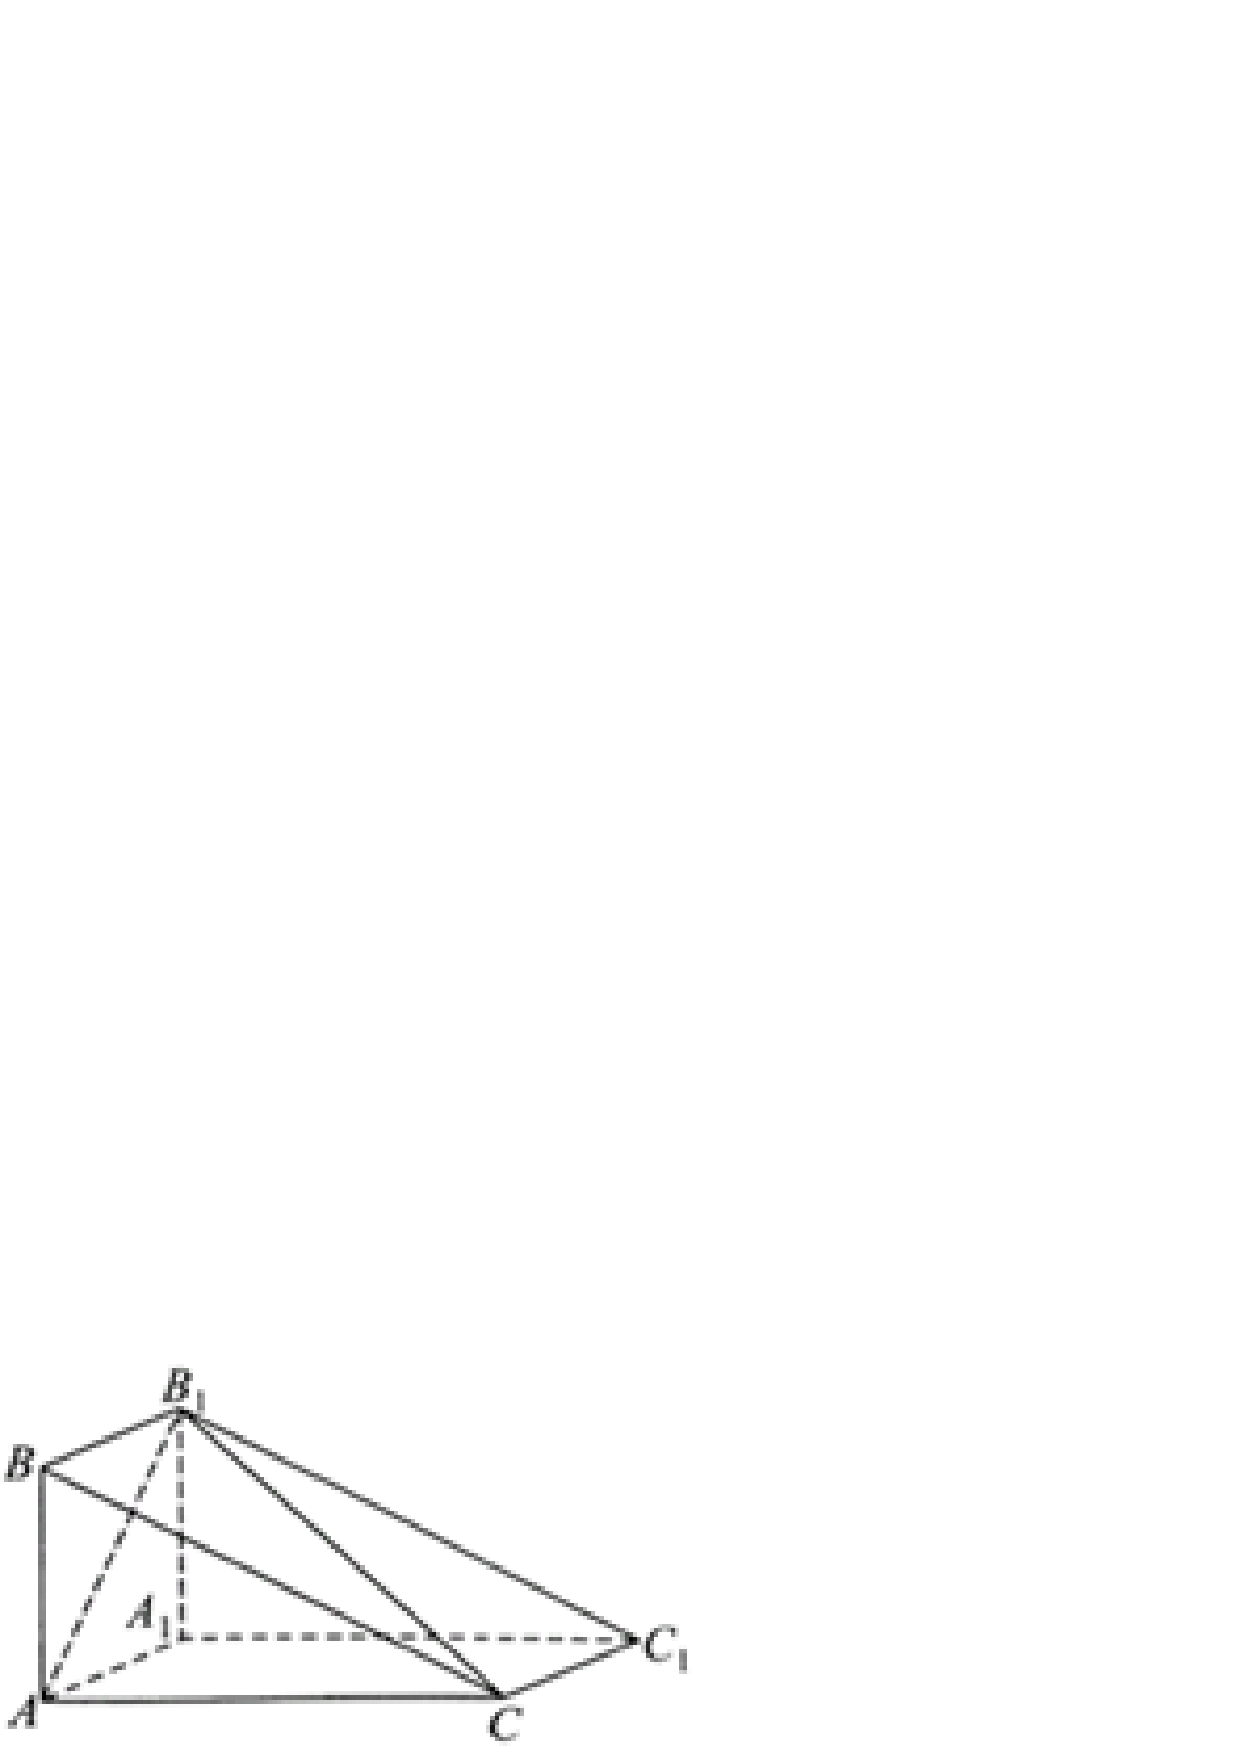
\includegraphics[width=0.53132in,height=0.21878in]{media/image156.png}

\textbf{【来源】}2015-2016学年贵州省凯里一中高二下期中数学试卷(带解析)

\textbf{【答案】}B

\textbf{【解析】}

由同向不等式的可加性可知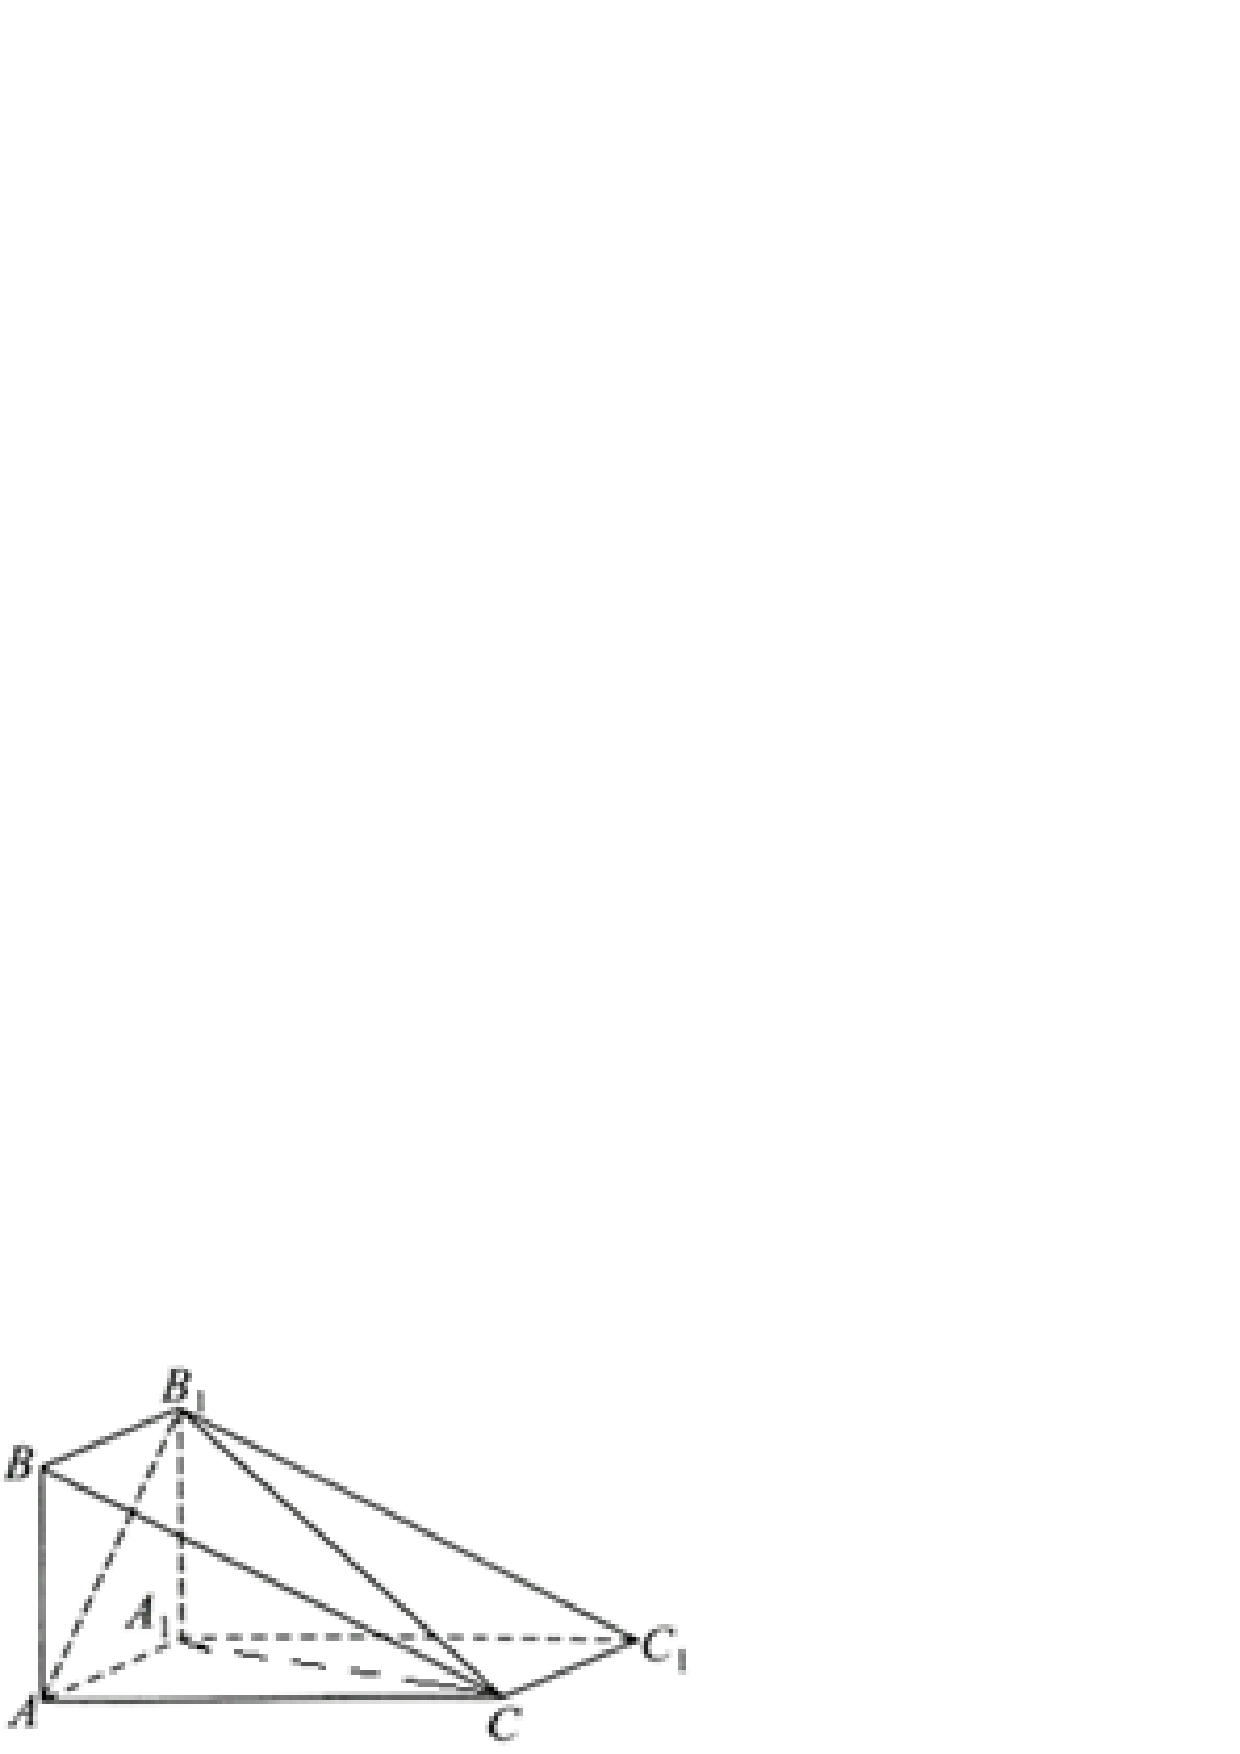
\includegraphics[width=0.38547in,height=0.19794in]{media/image157.png},
\includegraphics[width=0.40631in,height=0.19794in]{media/image158.png}
\includegraphics[width=1.03139in,height=0.19794in]{media/image159.png}成立.故选B.

考点:不等式的基本性质.

\textbf{15.如果}\includegraphics[width=0.63551in,height=0.19794in]{media/image160.png}\textbf{,那么下列各式一定成立的是(
)}

\textbf{A.}
\includegraphics[width=0.62509in,height=0.19794in]{media/image161.png}
\textbf{B.}\includegraphics[width=0.54174in,height=0.19794in]{media/image162.png}
\textbf{C.}
\includegraphics[width=0.51049in,height=0.21878in]{media/image163.png}
\textbf{D.}
\includegraphics[width=0.44798in,height=0.42714in]{media/image164.png}

\textbf{【来源】}2015-2016学年青海平安一中高二4月月考文科数学试卷(带解析)

\textbf{【答案】}C

\textbf{【解析】}

试题分析:A中应为\includegraphics[width=0.63551in,height=0.19794in]{media/image165.png},B中当
\includegraphics[width=0.38547in,height=0.19794in]{media/image166.png}时不成立,D应为
\includegraphics[width=0.4584in,height=0.42714in]{media/image167.png},故应选C.

考点:不等式的性质.

\textbf{16.已知整数a,b,c,t满足:2\textsuperscript{a}+2\textsuperscript{b}=2\textsuperscript{c},t=}\(\frac{a + b}{c}\)\textbf{,则log\textsubscript{2}t的最大值是(
)}

\textbf{A.0 B.log\textsubscript{2}3 C.2 D.3}

\textbf{【来源】}2015届四川省成都市第七中学高三一诊模拟理科数学试卷(带解析)

\textbf{【答案】}C

\textbf{【解析】}

不妨设a≤b,\(2^{b} < 2^{c} = 2^{a} + 2^{b} \leq 2^{b} + 2^{b} = 2^{b + 1} \Rightarrow b < c \leq b + 1\),

∵b,c∈Z,∴c=b+1,

\(\therefore 2^{b + 1} = 2^{a} + 2^{b}\)
\(\Rightarrow a = b = c - 1\).\(\therefore t = \frac{a + b}{c}\)
\(= 2 - \frac{2}{c}\).

∵a,t∈Z,∴c=±1,±2,∴t=0,1,3,4,故\({(\log_{2}t)}_{\max} = \log_{2}4 = 2\).

考点:指数与对数性质,不等式

\textbf{17.若a=2\textsuperscript{0.6},b=log\textsubscript{2}2,c=ln0.6,则(
)}

\textbf{A.a>b>c B.b>a>c C.c>a>b D.b>c>a}

\textbf{【来源】}2015-2016学年江西省高安中学高一重点上期中数学卷(带解析)

\textbf{【答案】}A

\textbf{【解析】}

试题分析:,故,故选A.

考点:指数与对数

\textbf{18.已知函数,若,,,则 (▲ )}

\textbf{A. B. C. D.}

\textbf{【来源】}2011届广东省华附、省实、广雅三校广州一模后联合适应性考试数学理卷

\textbf{【答案】}B

\textbf{【解析】}

本题考查函数的单调性.利用函数单调性比较数的大小.

因为,且函数是减函数,所以

即故选B

\textbf{19.设,,,则( )}

\textbf{A. B. C. D.}

\textbf{【来源】}安徽省阜阳市太和第一中学2020-2021学年高三上学期第一次校本教材反馈测试数学(文)试题

\textbf{【答案】}B

\textbf{【解析】}

【分析】

根据指数函数的单调性判断,再由作商法判断.

【详解】

因为函数是减函数,所以,所以

,所以,

所以

故选:B

【点睛】

本题主要考查了利用指数函数的单调性比较大小,属于中档题.

\textbf{20.下列不等式一定成立的是( )}

\textbf{A. B.}

\textbf{C. D.}

\textbf{【来源】}宁夏六盘山高级中学2019-2020学年高二上学期期中数学(理)试题

\textbf{【答案】}C

\textbf{【解析】}

【分析】

利用不等式的性质及基本不等式依次判断各选项即可得出.

【详解】

解:对于:,,故不成立;

对于:当时,当且仅当时取等号;

当时,当且仅当时取等号;故错误;

对于:,,故正确.

对于:等价于,即,故得,而题设,当时不成立.故错误;

故选:

【点睛】

本题考查了基本不等式的性质,考查了灵活解决问题的能力,属于基础题.

\textbf{21.已知,,则的取值范围是(  )}

\textbf{A. B. C. D.}

\textbf{【来源】}广东省潮州市2019届高三第二次模拟考试数学(理)试题

\textbf{【答案】}C

\textbf{【解析】}

【分析】

利用待定系数法求得,由,,结合,从而可得结果.

【详解】

令

则,

∴,

又,\ldots∴①

,

∴\ldots②

∴①②得.

则.

故选C.

【点睛】

本题主要考查不等式的性质以及指数函数的性质,意在考查综合运用所学知识解答问题的能力,属于中档题.

\textbf{22.已知等比数列满足,则的取值范围是( )}

\textbf{A. B. C. D.}

\textbf{【来源】}第十九篇求参数范围02---2020年高考数学选填题专项测试(文理通用)

\textbf{【答案】}D

\textbf{【解析】}

【分析】

设公比为\emph{q},根据等比数列的通项公式可得,①,,②,,③,再根据不等式的性质可得结果.

【详解】

设公比为\emph{q},∵\emph{a}\textsubscript{1}∈(0,1),\emph{a}\textsubscript{2}∈(1,2),\emph{a}\textsubscript{3}∈(3,4),

所以,①

,②

,③

所以,④

③×④得,⑤

由①得⑥,由③得⑦,

,得或⑧,

由⑤⑧可得:,

因为\emph{a}\textsubscript{4}=\emph{a}\textsubscript{3}\emph{q},∴..

故选:D

【点睛】

本题考查了等比数列的通项公式,考查了不等式的性质,属于中档题.

\textbf{23.若\emph{a}、\emph{b}、,且,则下列不等式中一定成立的是( )}

\textbf{A. B. C. D.}

\textbf{【来源】}江西省新余市第四中学2017-2018学年高二上学期期末数学(理)试题

\textbf{【答案】}D

\textbf{【解析】}

【分析】

利用不等式的性质证明,或者构造反例说明,即得解.

【详解】

由题意可知,\emph{a}、\emph{b}、,且

\emph{A}.若,满足,则,故本选项不正确;

\emph{B}.若,满足,则,故本选项不正确;

\emph{C}. 若,则,故本选项不成立;

\emph{D}.

故选:\emph{D}

【点睛】

本题考查了利用不等式的性质,判断代数式的大小,考查了学生综合分析,转化与划归的能力,属于基础题.

\textbf{24.下列不等式:①﹔②;③;④,其中恒成立的是( )}

\textbf{A.①④ B.③④ C.②③ D.①②}

\textbf{【来源】}沪教版(上海)高一第一学期新高考辅导与训练第2章不等式2.8基本不等式及其应用(1)

\textbf{【答案】}C

\textbf{【解析】}

【分析】

结合不等式的性质逐个验证.

【详解】

①当时,,不成立;

②因为,所以成立;

③易知,若,则,;

若,则,.

所以成立;

④,当或\emph{a},\emph{b}中仅有一个为0时成立,当时不成立.

故选:C

【点睛】

本题考查不等式的性质,属于基础题.

\textbf{25.设,给出下列三个结论:①;②;③.其中所有的正确结论的序号是 (
)}

\textbf{A.①③ B.①② C.②③ D.①②③}

\textbf{【来源】}福建省福州八县一中2018-2019学年高二上学期期中考试数学(理)试题

\textbf{【答案】}B

\textbf{【解析】}

【分析】

由题意逐一分析所给的说法是否正确即可.

【详解】

逐一分析所给的不等式:

由于,故,结合可得,说法①正确;

由于,故幂函数在区间上单调递减,结合可得,说法②正确;

由于,故,

对数函数单调递减,故,说法③错误.

综上可得:所有的正确结论的序号是①②.

本题选择\emph{B}选项.

【点睛】

本题主要考查不等式的性质,对数函数的单调性,幂函数的单调性等知识,意在考查学生的转化能力和计算求解能力.

\textbf{26.已知a=log\textsubscript{2}3.6,b=log\textsubscript{4}3.2,c=log\textsubscript{4}3.6,则(
).}

\textbf{A.a\textgreater b\textgreater c
B.a\textgreater c\textgreater b}

\textbf{C.b\textgreater a\textgreater c
D.c\textgreater a\textgreater b}

\textbf{【来源】}2013届浙江省温州市龙湾中学高三上学期期初考试文科数学试卷(带解析)

\textbf{【答案】}B

\textbf{【解析】}

试题分析:利用换底公式可得a=log\textsubscript{2}3.6=log\textsubscript{4}3.6\textsuperscript{2},然后根据对数函数y=log\textsubscript{4}x在(0,+∞)的单调性可进行比较即可.

解:∵a=log\textsubscript{2}3.6=log\textsubscript{4}3.6\textsuperscript{2}

∵y=log\textsubscript{4}x在(0,+∞)单调递增,

又∵3.6\textsuperscript{2}>3.6>3.2∴log\textsubscript{4}3.6\textsuperscript{2}>log\textsubscript{4}3.6>log\textsubscript{4}3.2

即a>c>b

故选B

点评:本题考查利用对数函数的单调性比较对数值大小,考查了换底公式的应用,是基础题.

\textbf{27. 设则下列判断中正确的是( )}

\textbf{A. B.}

\textbf{C. D.}

\textbf{【来源】}2016届黑龙江省大庆实验中学高三12月月考理科数学试卷(带解析)

\textbf{【答案】}B

\textbf{【解析】}

试题分析:令,则,故选B.

考点:特殊值法.

\textbf{28.已知函数,若,,则}

\textbf{A. B.}

\textbf{C. D.与的大小不能确定}

\textbf{【来源】}2011届浙江省杭州学军中学高三第一次月考理科数学卷

\textbf{【答案】}A

\textbf{【解析】}

【分析】

【详解】

\includegraphics[width=3.83333in,height=4.07292in]{media/image305.png}

故选A.

\textbf{29.甲、乙两人连续两天在同一个水果店购买了同一品种的砂糖橘,两天的价格不同,两人购买的方式不同,每人每天购买1次,甲每次总是买5斤,乙每次总是买20元的,设甲两次购买的平均价格为\emph{x}元斤,乙两次购买的平均价格为\emph{y}元斤,则下列关系式一定成立的是(
)}

\textbf{A. B.}

\textbf{C. D.}

\textbf{【来源】}陕西省西安中学2020-2021学年高三上学期第二次月考数学(文)试题

\textbf{【答案】}D

\textbf{【解析】}

【分析】

由题意求出得到的大小关系,然后由不等式的性质,对数函数,正弦函数的性质判断.

【详解】

设砂糖橘第一天的价格是元/斤,第二天价格是元/斤,,,

则,,

∵,∴,即,

∴,,A错;;B错;

在上不是单调函数,C错;

,∴,D正确.

故选:D.

【点睛】

本题考查不等式的性质,考查对数函数,正弦函数的性质,掌握作差法比较两实数的大小是解题基础.

\textbf{30.实数,,满足,,若,则( )}

\textbf{A. B. C. D.}

\textbf{【来源】}2.2综合拔高练

\textbf{【答案】}B

\textbf{【解析】}

【分析】

由题分析,三个数中必然一个为正,两个为负,可设,则,,先对进行通分,得,通过判断分子的正负即可求解

【详解】

因为且,所以不妨设,则,,

则.

因为,,所以,又,

所以,又,所以.

故选:B.

【点睛】

本题考查分式的正负判断,通过合理变形和代换是解题关键,属于中档题

\textbf{31.若,则下列不等式不成立的是( )}

\textbf{A. B.}

\textbf{C. D.}

\textbf{【来源】}2.1不等式的基本性质(2)

\textbf{【答案】}B

\textbf{【解析】}

【分析】

利用不等式的基本性质,对选项逐一分析,选出正确选项

【详解】

由,

选项A:利用数轴可得,则,根据不等式的性质,,则,故A成立;

选项B:由于,根据``如果,那么''可得,故B不成立;

选项C:由于,两边同乘,可得,对,对其左右两边同乘,得,即,故,即,故C成立;

选项D:,,故,故D成立;综上,选B

【点睛】

本题考查不等关系与不等式,考查熟练运用不等式的基本性质灵活证明命题的能力。

\textbf{32.设,.下列说法正确的是( )}

\textbf{A.则 B.则}

\textbf{C.则 D.则}

\textbf{【来源】}杭州新东方高一数学试卷224

\textbf{【答案】}B

\textbf{【解析】}

【分析】

举反例说明C,D不成立,再根据函数单调性,进而确定选项.

【详解】

因为所以CD不成立;

因为在上单调递增,所以由得,

故选:B

【点睛】

本题考查利用函数单调性判断命题真假,考查基本分析判断能力,属基础题.

\textbf{33.设 则下列关系正确的是}

\textbf{A. B. C. D.}

\textbf{【来源】}湖北省沙市中学2018-2019学年高一12月月考数学试题

\textbf{【答案】}C

\textbf{【解析】}

【分析】

由幂函数,指数函数,对数函数的单调性以及不等式的性质判断即可.

【详解】

A.,由幂函数 当函数在上单调递减,可知A错误;

由,由不等式的性质可得,故B错误;由指数函数
当函数在上单调递减,可知C正确;由对函数 当函数在上单调递减,可知D错误.

故选 C .

【点睛】

本题考查幂函数,指数函数,对数函数的单调性以及不等式的性质,属基础题.

\textbf{34.已知,则下列不等式一定成立的是}

\textbf{A. B. C. D.}

\textbf{【来源】}天津市和平区2019届高三下学期第一次质量调查数学(文)试题

\textbf{【答案】}D

\textbf{【解析】}

【分析】

由可得,故,据此逐一考查所给的选项是否正确即可.

【详解】

由可得,故,逐一考查所给的选项:

\emph{A}.;

\emph{B}.,的符号不能确定;

\emph{C}.;

\emph{D}..

本题选择\emph{D}选项.

【点睛】

本题主要考查对数函数的性质,不等式的性质及其应用等知识,意在考查学生的转化能力和计算求解能力.

\textbf{35.对于任意实数\emph{a},\emph{b},\emph{c},\emph{d},有下列命题:}

\textbf{①若\emph{a}\textgreater{}\emph{b},\emph{c}≠0,则\emph{ac}\textgreater{}\emph{bc};②若\emph{ac}\textsuperscript{2}\textgreater{}\emph{bc}\textsuperscript{2},则\emph{a}\textgreater{}\emph{b};}

\textbf{③若\emph{a}\textgreater{}\emph{b},则;④若\emph{a}\textgreater{}\emph{b}\textgreater0,\emph{c}\textgreater{}\emph{d},则\emph{ac}\textgreater{}\emph{bd}.}

\textbf{其中真命题的个数是( )}

\textbf{A.1 B.2 C.3 D.4}

\textbf{【来源】}2.1 命题、定理、定义 学案-苏教版高中数学必修第一册

\textbf{【答案】}A

\textbf{【解析】}

【分析】

根据不等式的性质作出判断即可.

【详解】

当\emph{c}\textless0时,①错误;\emph{ac}\textsuperscript{2}\textgreater{}\emph{bc}\textsuperscript{2},显然\emph{c}\textsuperscript{2}\textgreater0,因此②正确;当\emph{a}\textgreater0\textgreater{}\emph{b}时,③错误;当\emph{a}=2,\emph{b}=1,\emph{c}=-1,\emph{d}=-2时,显然④错误

故选:A

【点睛】

本题主要考查了判断命题的真假,涉及了不等式性质的应用,属于中档题.

\textbf{36.下列结论正确的是( )}

\textbf{A.若,则 B.若,则}

\textbf{C.若,则 D.若,则}

\textbf{【来源】}湖北省武汉市外国语学校2019-2020学年高一下学期5月月考数学试题

\textbf{【答案】}C

\textbf{【解析】}

【分析】

取特殊值判断ABD,根据不等式的性质判断C.

【详解】

对于A,取时,,则A错误;

对于B,取时,,则B错误;

对于C,因为,所以由不等式的性质可知,则C正确;

对于D,取时,,则D错误;

故选:C

【点睛】

本题主要考查了根据所给条件判断不等式是否成立,属于中档题.

\textbf{37.设,且,,,则与的大小关系为( ).}

\textbf{A. B. C. D.不确定}

\textbf{【来源】}沪教版(上海)高三年级新高考辅导与训练第二章不等式二、不等式证明

\textbf{【答案】}B

\textbf{【解析】}

【分析】

,讨论和两种情况,根据对数函数单调性得到答案.

【详解】

,

当时,,函数单调递增,故;

当时,,函数单调递减,故;

综上所述:.

故选:B.

【点睛】

本题考查了比较对数式的大小,意在考查学生的计算能力和分类讨论能力,利用函数单调性是解题的关键.

\textbf{38.下列命题正确的是}

\textbf{A.若 a>b,则a\textsuperscript{2}>b\textsuperscript{2}
B.若a>b,则 ac>bc}

\textbf{C.若a>b,则a\textsuperscript{3}>b\textsuperscript{3}
D.若a\textgreater b,则 <}

\textbf{【来源】}领军考试2018届高三阶段性测评(四)晋豫省际大联考(12月)
数学(理)

\textbf{【答案】}C

\textbf{【解析】}

对于,若,,则不成立;对于,若,则不成立;对于,若,则,则正确;对于,,,则不成立.

故选C

\textbf{39.,,下列命题正确的是( )}

\textbf{A.若,则 B.若,则}

\textbf{C.若,则 D.若,则}

\textbf{【来源】}山东省潍坊市第七中学2017-2018学年高二上学期期中考试数学试题

\textbf{【答案】}B

\textbf{【解析】}

当,则,则,故错误;当时,必有,则可得,故正确;令,则,满足,但,故错误;令,则,但,故错误,故选B.

\textbf{40.若}\includegraphics[width=0.65634in,height=0.19794in]{media/image417.png}\textbf{.则下列不等式中成立的是(
)}

\textbf{A.}\includegraphics[width=0.54174in,height=0.28129in]{media/image418.png}
\textbf{B.}\includegraphics[width=0.38547in,height=0.42714in]{media/image419.png}
\textbf{C.}\includegraphics[width=0.90638in,height=0.25003in]{media/image420.png}
\textbf{D.}\includegraphics[width=0.44798in,height=0.42714in]{media/image421.png}

\textbf{【来源】}广西桂林中学2017-2018学年高二上学期期中考试数学(文)试题

\textbf{【答案】}A

\textbf{【解析】}

,,所以B,D错误,

∵ ,∴ C错误,故选A.

\textbf{41.设x,y,z是互不相等的正数,则下列不等式中不恒成立的是( )}

\textbf{A.}

\textbf{B.}

\textbf{C.}

\textbf{D.}

\textbf{【来源】}2016届湖北襄阳五中高三5月二模文科数学试卷(带解析)

\textbf{【答案】}C

\textbf{【解析】}

【分析】

【详解】

试题分析:,故D恒成立;

由于函数,在单调递减;在单调递增, 当时,

即,当,即正确,即A正确;

由于,故B恒成立,

若,不等式不成立, 故C不恒成立,故选C.

考点:1、基本不等式证明不等式;2、单调性证明不等式及放缩法证明不等式.

\textbf{42.设,则的大小顺序是 ( )}

\textbf{A. B. C. D.}

\textbf{【来源】}松原市乾安县第七中学2016-2017学年高二下学期期末考试数学(文)试题

\textbf{【答案】}C

\textbf{【解析】}

三个数不能直接比较大小的,又因为三个数均为正数,所以平方之后再比较大小

所以,,所以,所以,选C.

\textbf{43.若,,则( )}

\textbf{A. B. C. D.}

\textbf{【来源】}2017届河北省石家庄市第二中学高三下学期模拟联考数学(文)试卷(带解析)

\textbf{【答案】}B

\textbf{【解析】}

由题意得,因为,则,

所以,故选B.

考点:实数指数幂的运算.

\textbf{44.若不等式}\(a > b\)\textbf{与}\(\frac{1}{a} > \frac{1}{b}\)\textbf{同时成立,则必有(
)}

\textbf{A.}\(a > b > 0\) \textbf{B.}\(0 > \frac{1}{a} > \frac{1}{b}\)
\textbf{C.}\(a > 0 > b\) \textbf{D.}\(\frac{1}{a} > \frac{1}{b} > 0\)

\textbf{【来源】}2013-2014学年河南省郑州一中高二上学期期中考试理科数学试卷(带解析)

\textbf{【答案】}C

\textbf{【解析】}

试题分析:因为两个不等式同时成立,利用2个等价关系可以得到a与b的关系.\(\because\frac{1}{a} > \frac{1}{b} \Rightarrow \frac{1}{a} - \frac{1}{b} > 0 \Rightarrow \frac{b - a}{\text{ab}} > 0\)又因为\(a > b\)所以\(ab < 0\).故答案为C

考点:不等式的性质

\textbf{45.对于非空集合A、B,定义运算:}\includegraphics[width=2.26073in,height=0.21878in]{media/image460.png}\textbf{.已知}\includegraphics[width=1.18767in,height=0.21878in]{media/image461.png}\textbf{,}\includegraphics[width=1.16683in,height=0.21878in]{media/image462.png}\textbf{,其中a、b、c、d满足}\includegraphics[width=0.88554in,height=0.19794in]{media/image463.png}\textbf{,}\includegraphics[width=0.82303in,height=0.19794in]{media/image464.png}\textbf{,则}\includegraphics[width=0.67718in,height=0.19794in]{media/image465.png}\textbf{(
)}

\textbf{A.}\includegraphics[width=0.91679in,height=0.21878in]{media/image466.png}
\textbf{B.}\includegraphics[width=0.91679in,height=0.21878in]{media/image467.png}

\textbf{C.}\includegraphics[width=0.8647in,height=0.23962in]{media/image468.png}
\textbf{D.}\includegraphics[width=0.8647in,height=0.23962in]{media/image469.png}

\textbf{【来源】}2015届广东省肇庆市高三第三次统一检测理科数学试卷(带解析)

\textbf{【答案】}D

\textbf{【解析】}

试题分析:本题可先由知M=\{x\textbar a<x<b\},N=\{x\textbar c<x<d\},其中a、b、c、d满足a+b=c+d,ab<cd<0,得到a,b,0,c,d的大小关系,再由新定义M⊕N的意义即可求出.

由已知M=\{x\textbar a<x<b\},∴a<b,又ab<0,∴a<0<b,同理可得c<0<d,

\(\because ab<cd<0,c<0,b>0,\therefore\frac{a}{c}>\frac{d}{b},\therefore\frac{a - c}{c}>\frac{d - b}{b},\)

\(\because a + b = c + d,\therefore a - c = d - b,\therefore\frac{d - b}{c}>\frac{d - b}{b},\)又∵c<0,b>0,∴d-b<0,因此,a-c<0,

∴a<c<0<d<b,∴M∩N=N,∴M⊕N=\{x\textbar a<x≤c,或d≤x<b\}=(a,c{]}∪{[}d,b).故选D.

考点:新定义、函数的性质,集合的运算、不等式的性质

\textbf{46.已知三角形的三边长分别为,设,则}

\textbf{与的大小关系是( )}

\textbf{A. B. C. D.}

\textbf{【来源】}20102011学年湖北省黄冈中学高二下学期期中考试文科数学卷

\textbf{【答案】}D

\textbf{【解析】}

【分析】

利用放缩法比较,利用作差法比较,从而可得结果.

【详解】

因为

所以,故选D.

【点睛】

本题主要考查``作差法''比较两个数的大小,属于简单题.
比较两个数的大小主要有四种方法:(1)作差法;(2)作商法;(3)函数单调性法;(4)基本不等式法.

\textbf{47.给出下列四个命题:}

\textbf{①若集合A,B满足,则;}

\textbf{②给定命题,若``\,''为真,则``\,''为真;}

\textbf{③设若,则;}

\textbf{④若直线与直线垂直,则.}

\textbf{其中正确命题的个数是}

\textbf{A.1 B.2 C.3 D.4}

\textbf{【来源】}烟台市中英文学校2010届高三一模考试文科数学试题

\textbf{【答案】}B

\textbf{【解析】}

【分析】

【详解】

因为,则,所以①正确;

若``\,''为真,则``\,''不一定为真,所以②错误;

若,则,所以③错误;

若直线与直线垂直,则,所以④正确

选B.

\textbf{48.下列命题正确的是( )}

\textbf{A.若,则 B.若,则}

\textbf{C.若,则 D.若,则}

\textbf{【来源】}宁夏回族自治区银川市宁夏育才中学2019-2020学年高二上学期期中数学(理)试题

\textbf{【答案】}D

\textbf{【解析】}

【分析】

\emph{A}项中,需要看分母的正负;\emph{B}项和\emph{C}项中,已知两个数平方的大小只能比较出两个数绝对值的大小.

【详解】

\emph{A}项中,若,则有,故\emph{A}项错误;\emph{B}项中,若,则,故\emph{B}项错误;\emph{C}项中,若则即,故\emph{C}项错误;\emph{D}项中,若,则一定有,故\emph{D}项正确.

故选:\emph{D}

【点睛】

本题主要考查不等关系与不等式,属于基础题.

\textbf{49.已知,给出下列命题:}

\textbf{①若,则; ②若,则;}

\textbf{③若,则; ④若,则.}

\textbf{其中真命题的个数是( )}

\textbf{A.1 B.2 C.3 D.4}

\textbf{【来源】}浙江省十校联盟2019-2020学年高三下学期寒假返校考试数学试题

\textbf{【答案】}B

\textbf{【解析】}

【分析】

①若,则,然后两边平方,再通过作差法即可得解;

②若,则,然后利用立方差公式可知,再结合以及不等式的性质即可判断;

③若,则,再利用,得出,从而求得的范围,进而判断;

④取特殊值,,即可判断.

【详解】

解:①若,

则,

所以,

所以,即①错误;

若,

则,

即,

因为,

所以,

所以,

所以,即,所以②正确;

若,

则,

因为,所以,

所以,即③正确;

④取,,满足,

但,所以④错误;

所以真命题有②③,

故选:B.

【点睛】

本题考查命题真假的判断,涉及根据不等式的性质证明不等式、指对运算法则、立方差公式等,考查学生的分析能力和运算能力.

\textbf{50.已知定义在上的函数,正实数满足,则( )}

\textbf{A. B. C. D.}

\textbf{【来源】}2020届陕西省安康市高三教学质量检测第四次联考数学(文)试题

\textbf{【答案】}C

\textbf{【解析】}

【分析】

求导可判断函数在上单调递增,即可得到,结合不等式的性质,可得到,进而可得出的大小关系.

【详解】

因为,所以函数在上单调递增,所以,

则,即,

又,所以.

由,可得;由可得,

所以.

故选:C.

【点睛】

本题考查函数单调性的应用,考查不等式的性质,考查学生的推理论证能力,属于中档题.

\textbf{51.是等比数列,是等差数列,,公差,公比,则与的大小关系为(
).}

\textbf{A. B. C. D.不确定}

\textbf{【来源】}沪教版(上海)高三年级新高考辅导与训练第四章数列与数学归纳法本章测试

\textbf{【答案】}C

\textbf{【解析】}

【分析】

先根据等差数列与等比数列通项公式求,再根据条件得,最后根据作差法,结合二项式定理放缩确定大小.

【详解】

所以

故选:C

【点睛】

本题考查等差数列与等比数列通项公式、作差法,二项式定理,考查综合分析论证能力,属中档题.

\textbf{52.已知点在直线上,且满足,则的取值范围为( )}

\textbf{A. B.}

\textbf{C. D.}

\textbf{【来源】}山东省泰安肥城市2020届高三适应性训练(一)数学试题

\textbf{【答案】}B

\textbf{【解析】}

【分析】

由,求出的取值范围,再求的范围.

【详解】

由题意,,

∵,∴,解得,

,

∵,∴或,

∴或,所以.

故选:B.

【点睛】

本题考查直线方程,考查不等式的性质,解题过程是利用点在直线上,且满足的不等关系求出的范围,然后再利用不等式的性质求解.

\textbf{53.若实数\emph{a}>\emph{b},则下列结论成立的是(   )}

\textbf{A.\emph{a}\textsuperscript{2}>\emph{b}\textsuperscript{2} B.
C.\emph{ln}2\emph{\textsuperscript{a}}>\emph{ln}2\emph{\textsuperscript{b}}
D.\emph{ax}\textsuperscript{2}>\emph{bx}\textsuperscript{2}}

\textbf{【来源】}四川省成都市温江区2018-2019学年高一下学期期末数学试题

\textbf{【答案】}C

\textbf{【解析】}

【分析】

特值法排除A,B,D,单调性判断C

【详解】

由题意,可知:

对于\emph{A}:当\emph{a}、\emph{b}都是负数时,很明显\emph{a}\textsuperscript{2}<\emph{b}\textsuperscript{2},故选项\emph{A}不正确;

对于\emph{B}:当\emph{a}为正数,\emph{b}为负数时,则有,故选项\emph{B}不正确;

对于\emph{C}:∵\emph{a}>\emph{b},∴2\emph{\textsuperscript{a}}>2\emph{\textsuperscript{b}}>0,∴\emph{ln}2\emph{\textsuperscript{a}}>\emph{ln}2\emph{\textsuperscript{b}},故选项\emph{C}正确;

对于\emph{D}:当\emph{x}=0时,结果不成立,故选项\emph{D}不正确;

故选:\emph{C}.

【点评】

本题主要考查不等式的性质应用,特殊值技巧的应用,指数函数、对数函数值大小的比较.本题属中档题.

\textbf{54.下列命题中,正确的是( )}

\textbf{A.若,,则 B.若,则}

\textbf{C.若,则 D.若,,则}

\textbf{【来源】}宁夏石嘴山市第一高级中学2019-2020学年高二上学期期末数学试题

\textbf{【答案】}C

\textbf{【解析】}

【分析】

利用不等式的基本性质进行逐项判断即可,不成立的举反例.

【详解】

对于选项A:若,满足,,但是不成立,故选项A错误;

对于选项B:若,满足,但不成立,故选项B错误;

对于选项C:因为,整理化简可得,因为,所以,即成立,故选项C正确;

对于选项D:若,满足,,但是不成立,故选项D错误;

【点睛】

本题考查不等式与不等关系;不等式的基本性质的灵活运用是求解本题的关键;属于中档题、常考题型.

\textbf{55.若,则下列不等式中不成立的是( )}

\textbf{A. B. C. D.\emph{a}\textsuperscript{5} +
\emph{b}\textsuperscript{5} \textless{}
\emph{a}\textsuperscript{2}\emph{b}\textsuperscript{3} +
\emph{a}\textsuperscript{3}\emph{b}\textsuperscript{2}}

\textbf{【来源】}福建省莆田市第一中学2018-2019学年高二上学期第一次月考数学(文)试题

\textbf{【答案】}B

\textbf{【解析】}

【分析】

根据不等式的性质判断A,C,根据作差法判断C,举反例判断B.

【详解】

由于a<b<0,则\textbar a\textbar>\textbar b\textbar,即,故A正确,

当a=-2,b=-1时, ,故B不正确,\\
由a<b<0,两边同时除以ab可得,故C正确,\\
,\\
故D正确.

故选B.

【点睛】

本题考查不等式的性质,解题的关键是利用不等式的性质,不正确结论,列举反例.

\textbf{56.已知,以下一定成立的是( )}

\textbf{A. B. C. D.}

\textbf{【来源】}浙江省宁波效实中学2018-2019学年高一上学期期中考试数学试题

\textbf{【答案】}D

\textbf{【解析】}

【分析】

根据不等式性质推导D,举反例说明A,B ,C不成立.

【详解】

2\textgreater1\textgreater0\textgreater-1\textgreater-2,21=-1(-2),2(-1)=1(-2),,A,B,C错;

因为,所以,因此,即得,D对.

【点睛】

本题考查不等式性质,考查基本分析判断能力.

\textbf{57.已知:,则3,,的大小关系是( )}

\textbf{A. B.}

\textbf{C. D.}

\textbf{【来源】}湖南省益阳市2019届高三4月模拟考试数学(理)试题

\textbf{【答案】}D

\textbf{【解析】}

【分析】

先将指数式化为对数式,再根据对数函数单调性以及运算法则比较大小,确定选项.

【详解】

,,

∴;

又 ,∴.故选D.

【点睛】

本题考查指数式化与对数式关系以及对数函数单调性,考查基本分析求解能力,属基础题.

\textbf{58.设,,,且,则( )}

\textbf{A. B. C. D.}

\textbf{【来源】}福建省漳州市2016-2017学年高一下学期期末考试数学试题

\textbf{【答案】}C

\textbf{【解析】}

若,则不成立,故答案A错误;若,则不成立,故答案B错误;因为,所以,则由不等式的性质对不等式两边同乘以可得
,即,故答案C 正确;若,则答案D不正确,应选答案C.

\textbf{59.已知,且,下列不等式中,一定成立的是 ( )}

\textbf{①;②;③;④}

\textbf{A.①② B.③④ C.②③ D.①④}

\textbf{【来源】}广东省中山一中2018届高三级第五次统测试卷理科数学试题

\textbf{【答案】}B

\textbf{【解析】}

,且当时,,

故① 错误; ,且,即,,故② 错误;,且 ,,故③ 正确;,且, ,故④
正确,故选B.

\textbf{60.已知且,则的取值范围是( )}

\textbf{A. B. C. D.}

\textbf{【来源】}浙江省台州市五校2019-2020学年高一下学期期中联考数学试题

\textbf{【答案】}B

\textbf{【解析】}

【分析】

由已知条件推导出,,再由得出,由得出,结合不等式的基本性质可求得的取值范围.

【详解】

,,则,,,则,

由得,则,即,即,

又,,因此,的取值范围是.

故选:B.

【点睛】

本题考查代数式取值范围的求解,考查不等式基本性质的应用,考查计算能力,属于中等题.

\textbf{61.设,且,则( )}

\textbf{A. B. C. D.}

\textbf{【来源】}安徽省亳州市第二中学2018-2019学年高二上学期期中数学(文)试题

\textbf{【答案】}C

\textbf{【解析】}

【分析】

取特殊值判断\emph{A,D},根据不等式的性质判断\emph{B},根据幂函数的性质判断\emph{C}.

【详解】

\emph{A}选项,取时,不等式不成立;

\emph{B}选项,不等式两边加上同一个数,不等号方向不发生改变,故错误;

\emph{C}选项,根据幂函数在R上为增函数知,故正确;

\emph{D}选项,取,不等式不成立,故错误.

故选:\emph{C}

【点睛】

本题主要考查了不等式的性质,幂函数的单调性,特值法,属于中档题.

\textbf{62.若\emph{a}>\emph{b},\emph{c}为实数,下列不等式成立是()}

\textbf{A.\emph{ac}>\emph{bc} B.\emph{ac}<\emph{bc} C. D.}

\textbf{【来源】}陕西省黄陵中学本部2018-2019学年高二下学期期末考试数学(文)试题

\textbf{【答案】}D

\textbf{【解析】}

【分析】

由已知条件,利用不等式的基本性质,直接求解,即可得到答案.

【详解】

由题意,为实数,

在A中,当时,不定成立,所以不正确;

在B中,当时,不定成立,所以不正确;

在C中,当时,不定成立,所以不正确;

在D中,因为,所以成立,故选D.

【点睛】

本题主要考查了不等式的基本性质的应用,其中解答中熟记不等式的基本性质,合理推理、运算是解答的关键,着重考查了推理与运算能力,属于基础题.

\textbf{63.对于实数\emph{a},\emph{b},\emph{c},给出下列命题:①若\emph{a}>\emph{b},则\emph{ac}\textsuperscript{2}>\emph{bc}\textsuperscript{2};②若0>\emph{a}>\emph{b},则;③若\emph{a}>\emph{b},,则\emph{a}>0,\emph{b}<0;④若\emph{a}>\emph{b}>\emph{c}>0,则.其中真命题的个数为(  )}

\textbf{A.0 B.1 C.2 D.3}

\textbf{【来源】}上海市建平中学2015-2016学年高一上学期期中数学试题

\textbf{【答案】}C

\textbf{【解析】}

【分析】

举例说明①错误;利用基本不等式的性质推得②正确;举例说明③错误;利用分析法说明④正确.

【详解】

①若\emph{a}>\emph{b},则\emph{ac}\textsuperscript{2}>\emph{bc}\textsuperscript{2},错误,当\emph{c}\textsuperscript{2}=0时,\emph{ac}\textsuperscript{2}=\emph{bc}\textsuperscript{2};

②若0>\emph{a}>\emph{b},则,把\emph{a}>\emph{b}两边同时乘以,得,即正确;

③当\emph{a}>\emph{b}>0或\emph{b}<\emph{a}<0时,有,③错误;

④\emph{a}>\emph{b}>\emph{c}>0,则\emph{a}+\emph{c}>0,\emph{b}+\emph{c}>0,若成立,则\emph{ab}+\emph{ac}>\emph{ab}+\emph{bc},即

\emph{ac}>\emph{bc},也就是\emph{a}>\emph{b},此时成立,故④正确.

所以真命题的个数是2.

故选:C

【点睛】

本题考查命题的真假判断与应用,考查了基本不等式的性质,属于基础题.

\textbf{64.已知实数,则下列不等关系中错误的是( )}

\textbf{A. B.}

\textbf{C. D.}

\textbf{【来源】}2020届重庆市巴蜀中学高考适应性月考卷(四)数学(理)试题

\textbf{【答案】}D

\textbf{【解析】}

【分析】

对每个不等式进行判断.也可举反例说明不成立.

【详解】

∵,

∴,A正确;

,B正确;

,C正确;

若,满足,但,D错误.

故选:D.

【点睛】

本题考查不等式的证明,不等式的证明可用作差法比较大小,也可用综合法进行证明,还可用反证法证明,如果不等式不成立可以举反例说明.

\textbf{65.若,,则  }

\textbf{A. B. C. D.}

\textbf{【来源】}四川省眉山一中办学共同体2019届高三10月月考数学(理)试卷

\textbf{【答案】}D

\textbf{【解析】}

【分析】

运用不等式对四个选项逐一分析

【详解】

对于,,,,则,故错误

对于,若,则,即,这与矛盾,故错误

对于,,,,则,故错误

对于,,,故正确

故选

【点睛】

本题考查了不等式的性质,由未知数的范围确定结果,属于基础题.

\begin{quote}
\textbf{66.设函数,若对任意恒成立,则实数x的取值范围是  }
\end{quote}

\textbf{A. B. C. D.}

\textbf{【来源】}山东省烟台市2018-2019学年高一上学期期中考试数学试题

\textbf{【答案】}B

\textbf{【解析】}

【分析】

将不等式左边构造为以为自变量的函数,其图象是直线,其最值在区间两端点处取得.

【详解】

因为,可化为:对任意恒成立,

令,则,即,解得:,

故选.

【点睛】

本题考查了不等式恒成立问,求解过程中运用了更换主元的方法,转化为直线问题,代入端点求出结果,属中档题.

\textbf{67.设,若,,则与的大小关系是( )}

\textbf{A. B. C. D.不能确定}

\textbf{【来源】}吉林省舒兰市第一高级中学校2018-2019学年高二下学期第一次月考数学(文)试题

\textbf{【答案】}B

\textbf{【解析】}

【分析】

对S和T进行分子有理化,然后通过作差比较即可得到结论.

【详解】

,

,

又,

所以S-T\textless0,即S\textless T

故选B

【点睛】

本题考查利用作差法比较大小关系,属于基础题.

\textbf{68.设,且,则( )}

\textbf{A. B. C. D.}

\textbf{【来源】}2014-2015学年福建省德化一中高二上学期第一次质检文科数学试卷(带解析)

【答案】D

\textbf{【解析】}

试题分析:A.,时不成立,B.,时不成立,C.

也不成立,D.只要,恒成立

考点:不等式成立问题.

\textbf{69.设,则的大小关系是}

\textbf{A. B. C. D.}

\textbf{【来源】}2014-2015学年山东省枣庄市四十二中高一上学期期中考试数学试卷(带解析)

\textbf{【答案】}B

【解析】

试题分析:因为,故

考点:指数函数、对数函数的图像和性质.

\textbf{70.若,则与的大小关系为( )}

\textbf{A. B. C. D.不能确定}

\textbf{【来源】}海南省海南中学1011学年高二下学期期末考试数学(文)

\textbf{【答案】}B

\textbf{【解析】}本题考查不等式性质;比较两个数的大小的方法:比较法

因为\includegraphics[width=1.00014in,height=0.21878in]{media/image728.png}所以

则所以故选B

\textbf{71.对于实数,``\,''是``\,''的( )}

\textbf{A.充分不必要条件 B.必要不充分条件}

\textbf{C.充要条件 D.既不充分也不必要条件}

\textbf{【来源】}四川省成都市龙泉第二中学2018届高三10月月考数学(文)试题

\textbf{【答案】}B

\textbf{【解析】}

由``\,''可得,即``\,''成立,若``\,'',
时``\,''不成立,所以``\,''是``\,''的必要不充分条件,故选B.

【方法点睛】本题通过主要考查不等式的性质以及充分条件与必要条件,属于中档题.判断充要条件应注意:首先弄清条件和结论分别是什么,然后直接依据定义、定理、性质尝试.对于带有否定性的命题或比较难判断的命题,除借助集合思想化抽象为直观外,还可利用原命题和逆否命题、逆命题和否命题的等价性,转化为判断它的等价命题;对于范围问题也可以转化为包含关系来处理.

\textbf{72.若,,则下列不等式不正确的是( )}

\textbf{A. B. C. D.}

\textbf{【来源】}山东省东营市河口区一中2017-2018学年度第二学期普通高中模块检查高二数学(文)试题

\textbf{【答案】}D

\textbf{【解析】}

分析:根据不等式性质推导,确定选项.

详解:因为,,所以

因为,,所以

因为,,所以

因为,,所以

选D.

点睛:本题考查不等式性质,考查基本推理论证能力.

\textbf{73.已知,为正实数,}

\textbf{①若,则;}

\textbf{②若,则;}

\textbf{③若,则;}

\textbf{④若,则;}

\textbf{上述命题中正确的是( )}

\textbf{A.①② B.②③ C.③④ D.①④}

\textbf{【来源】}河南省郑州市第一中学网校2017-2018学年高二上学期期中联考数学(理)试题

\textbf{【答案】}D

\textbf{【解析】}

若,不妨取,此时;说法②错误,排除\emph{AB}选项,

若,不妨取,此时;说法③错误,排除\emph{C}选项,

本题选择\emph{D}选项.

\textbf{74.下列说法正确的是(  )}

\textbf{A.``}\(x < 1\)\textbf{''是``}\(\log_{2}\left( x + 1 \right) < 1\)\textbf{''的充分不必要条件}

\textbf{B.命题``}\(\forall x > 0\)\textbf{,}\(2^{x} > 1\)\textbf{''的否定是``}\(\exists x_{0} \leq 0\)\textbf{,}\(2^{x_{0}} \leq 1\)\textbf{''}

\textbf{C.命题``若}\(a \leq b\)\textbf{,则}\(ac^{2} \leq bc^{2}\)\textbf{''的逆命题为真命题}

\textbf{D.命题``若}\(a + b \neq 5\)\textbf{,则}\(a \neq 2\)\textbf{或}\(b \neq 3\)\textbf{''为真命题}

\textbf{【来源】}2017届云南省云南师范大学附属中学高三高考适应性月考(五)文数试卷(带解析)

\textbf{【答案】}D

\textbf{【解析】}

选项A:\(\log_{2}(x + 1) < 1 \Leftrightarrow 0 < x + 1 < 2 \Leftrightarrow - 1 < x < 1\),所以``\(x < 1\)''是其必要不充分条件;选项B:命题``\(\forall x > 0,\text{  }2^{x} > 1\)''的否定是``\(\exists x_{0} > 0,\text{  }2^{x_{0}} \leq 1\)'';选项C:命题``若\(a \leq b\),则\(ac^{2} \leq bc^{2}\)''的逆命题是``若\(ac^{2} \leq bc^{2}\),则\(a \leq b\)'',当\emph{c}=0时,不成立;选项D:其逆否命题为``若\(a = 2\)且\(b = 3\),则\(a + b = 5\)''为真命题,故原命题为真,故选D.

\textbf{75.已知,则的取值范围是 (   )}

\textbf{A. B. C. D.}

\textbf{【来源】}黑龙江省双鸭山市第一中学2017-2018学年高二4月月考数学(文)试题

\textbf{【答案】}C

\textbf{【解析】}

设

易得:,

∴

故选:C

点睛:根据不等式组确定二元目标式范围的方程有二,其一:利用待定系数法表示目标,直接加减一次即可;其二:利用线性规划的方法处理.

\textbf{76.实数,,满足且,则下列关系式成立的是( )}

\textbf{A. B. C. D.}

\textbf{【来源】}贵阳第一中学2018届高考适应性月考卷(七)理数

\textbf{【答案】}A

\textbf{【解析】}

∵∴由∴∴综上,可得 .

故选A.

\textbf{77.设集合则``\,''是``\,''的( )}

\textbf{A.充要条件 B.必要不充分条件}

\textbf{C.充分不必要条件 D.既不充分也不必要条件}

\textbf{【来源】}甘肃省兰州市第一中学2016-2017学年高二下学期期末考试数学(文)试题

\textbf{【答案】}C

\textbf{【解析】}

试题分析:,,∵,选C.

考点:1、分式不等式和绝对值不等式的解法;2、充分条件和必要条件.

\textbf{78.
已知\emph{a}=,\emph{b}=,\emph{c}=,则实数a,b,c的大小关系是(  )}

\textbf{A.a\textgreater c\textgreater b
B.b\textgreater a\textgreater c}

\textbf{C.a\textgreater b\textgreater c
D.c\textgreater b\textgreater a}

\textbf{【来源】}人教A版高中数学 高三二轮(文)专题04
基本初等函数、函数与方程 测试

\textbf{【答案】}C

\textbf{【解析】}

依题意得,

∴,

∴,

又,

∴.选\emph{C}.

\textbf{79.给出下列命题:
①若}\(a,b \in R_{+},a \neq b\)\textbf{,则}\(a^{3} + b^{3} > a^{2}b + ab^{2}\)\textbf{;
②若}\(a,b,m \in R_{+},a < b\)\textbf{,则}
\(\frac{a + m}{b + m} < \frac{a}{b}\)\textbf{;
③若}\(\frac{a}{c^{2}} > \frac{b}{c^{2}}\)\textbf{,则}\(a > b\)\textbf{;
④当}\(x \in \left( 0,\frac{\pi}{2} \right)\)\textbf{时,}\(\sin x + \frac{2}{\sin x}\)\textbf{的最小值为}\(2\sqrt{2}\)\textbf{,其中结论正确的个数为(
)}

\textbf{A.}\(1\) \textbf{B.}\(2\) \textbf{C.}\(3\) \textbf{D.}\(4\)

\textbf{【来源】}山东省济南第一中学2019-2020学年高二10月阶段性检测数学试题

\textbf{【答案】}B

\textbf{【解析】}

【分析】

对于①②利用作差法可证明不等式是否成立,对于③由不等式性质可判断,对于④由基本不等式求得最值,并判断等号能否取到即可.

【详解】

对于①,若\(a,b \in R_{+},a \neq b\),则\(\left( a^{3} + b^{3} \right) - \left( a^{2}b + ab^{2} \right) = \left( a - b \right)^{2}\left( a + b \right) > 0\)成立,即\(a^{3} + b^{3} > a^{2}b + ab^{2}\)成立,所以①正确;

对于②,若\(a,b,m \in R_{+},a < b\),则\(\frac{a + m}{b + m} - \frac{a}{b} = \frac{m\left( a - b \right)}{b\left( b + m \right)} > 0\),即\(\frac{a + m}{b + m} < \frac{a}{b}\)不成立,所以②错误;

对于③,若\(\frac{a}{c^{2}} > \frac{b}{c^{2}}\),由不等式性质两边同时乘以\(c^{2}\),可得\(a > b\),所以③正确;

对于④,当\(x \in \left( 0,\frac{\pi}{2} \right)\)时,\(\sin x + \frac{2}{\sin x} \geq 2\sqrt{2}\),当且仅当\(\sin x = \frac{2}{\sin x}\)时取等号,因为\(\sin x = \sqrt{2}\)不成立,所以④错误;

综上可知,正确的为①③;

故选:B.

【点睛】

本题考查了作差法证明不等式是否成立,不等式性质应用,基本不等式求最值及等号成立条件,属于中档题.

\textbf{80.设,则下列不等式中一定成立的是( )}

\textbf{A. B. C. D.}

\textbf{【来源】}河南省信阳市息县第一高级中学2019-2020学年高二上学期第三次阶段性考试数学(文)试题

\textbf{【答案】}C

\textbf{【解析】}

【分析】

根据不等式的性质以及特殊值法进行判断即可.

【详解】

由,得出,故A错误;

当时,,,故BD错误;

由基本不等式得,即,故C正确;

故选:C

【点睛】

本题主要考查了由已知条件判断所给不等式是否成立,属于中档题.

\textbf{81.已知,满足,则的取值范围是( )}

\textbf{A. B. C. D.}

\textbf{【来源】}安徽省六安市第一中学2017-2018学年高一下学期期末考试数学(理)试题

\textbf{【答案】}A

\textbf{【解析】}

分析:该问题是已知不等关系求范围的问题,可以用待定系数法来解决.

详解:设α+3β=λ(α+β)+v(α+2β)

=(λ+v)α+(λ+2v)β.

比较α、β的系数,得,

从而解出λ=﹣1,v=2.

分别由①、②得﹣1≤﹣α﹣β≤1,2≤2α+4β≤6,

两式相加,得1≤α+3β≤7.

故α+3β的取值范围是{[}1,7{]}.

故选A

点睛:本题考查待定系数法,考查不等式的基本性质,属于基础题.

\textbf{82.两个正实数,满足,,成等差数列,则不等式恒成立时实数的取值范围是(
)}

\textbf{A. B. C. D.}

\textbf{【来源】}福建省龙岩市一级达标校2019-2020学年高一下学期期末质检数学试题

\textbf{【答案】}C

\textbf{【解析】}

【分析】

由题意利用等差数列的定义和性质求得,再利用基本不等式求得,根据题意,,由此求得的范围.

【详解】

解:两个正实数,满足,,成等差数列,

,,,.

不等式恒成立,即恒成立,

即恒成立.

,求得,

故选:C.

【点睛】

本题主要考查等差数列的定义和性质,不等式的恒成立问题,基本不等式的应用,属于基础题.

\textbf{83.设,则下列结论中正确的是( )}

\textbf{A. B. C. D.}

\textbf{【来源】}河南省豫北重点中学2017-2018学年高二12月联考数学(理)试卷

\textbf{【答案】}D

\textbf{【解析】}

【分析】

【详解】

,A错误

当时;B错误;

当时 ;C错误;

成立;所以选D.

\textbf{84.若a>0,b>0,且a+b=4,则下列不等式中恒成立的是( )}

\textbf{A.}\includegraphics[width=0.18758in,height=0.36473in]{media/image843.png}\textbf{>}\includegraphics[width=0.10421in,height=0.36473in]{media/image844.png}
\textbf{B.}\includegraphics[width=0.10421in,height=0.36473in]{media/image845.png}\textbf{+}\includegraphics[width=0.10421in,height=0.36473in]{media/image846.png}\textbf{≤1
C.}\includegraphics[width=0.29178in,height=0.18758in]{media/image847.png}\textbf{≥2
D.}\includegraphics[width=0.48978in,height=0.42726in]{media/image848.png}\textbf{≤}\includegraphics[width=0.10421in,height=0.36473in]{media/image849.png}

\textbf{【来源】}{[}同步{]}2014年新人教B版选修4-5
1.2基本不等式练习卷(带解析)

\textbf{【答案】}D

\textbf{【解析】}

试题分析:由题设知ab≤\includegraphics[width=0.92746in,height=0.42726in]{media/image850.png},所以\includegraphics[width=0.47936in,height=0.36473in]{media/image851.png},\includegraphics[width=0.87535in,height=0.36473in]{media/image852.png},\includegraphics[width=0.56273in,height=0.18758in]{media/image853.png},\includegraphics[width=0.48978in,height=0.42726in]{media/image854.png}=\includegraphics[width=1.13588in,height=0.4481in]{media/image855.png}=\includegraphics[width=0.60441in,height=0.39599in]{media/image856.png}≤\includegraphics[width=0.10421in,height=0.36473in]{media/image857.png},由此能够排除选项A、B、C,从而得到正确选项.

解:∵a>0,b>0,且a+b=4,

∴ab≤\includegraphics[width=0.92746in,height=0.42726in]{media/image858.png},

∴\includegraphics[width=0.47936in,height=0.36473in]{media/image859.png},故A不成立;

\includegraphics[width=0.87535in,height=0.36473in]{media/image860.png},故B不成立;

\includegraphics[width=0.56273in,height=0.18758in]{media/image861.png},故C不成立;

∵ab≤4,a+b=4,∴16﹣2ab≥8,

∴\includegraphics[width=0.48978in,height=0.42726in]{media/image862.png}=\includegraphics[width=1.13588in,height=0.4481in]{media/image863.png}=\includegraphics[width=0.60441in,height=0.39599in]{media/image864.png}≤\includegraphics[width=0.10421in,height=0.36473in]{media/image865.png},故D成立.

故选D.

考点:基本不等式.

\textbf{85.小茗同学的妈妈是吉林省援鄂医疗队的队员,为了迎接凯旋归来的英雄母亲,小茗准备为妈妈献上一束鲜花.据市场调查,已知6枝玫瑰花与3枝康乃馨的价格之和大于24元,而4枝玫瑰花与5枝康乃馨的价格之和小于22元,则2枝玫瑰花的价格和3枝康乃馨的价格比较结果是(
)}

\textbf{A.3枝康乃馨价格高 B.2枝玫瑰花价格高 C.价格相同 D.不确定}

\textbf{【来源】}吉林省长春实验中学2019-2020学年高一6月月考数学(理)试题

\textbf{【答案】}B

\textbf{【解析】}

【分析】

设1枝玫瑰和1枝康乃馨的价格分别元,由题意可得:,令,根据待定系数法求得,借助不等式性质即可证得.

【详解】

设1枝玫瑰和1枝康乃馨的价格分别元,由题意可得:,

令,

则,解得:

,

因此.

所以2枝玫瑰的价格高.

故选:B

【点睛】

本题考查不等关系与不等式性质,考查不等式比较大小的问题,属于中档题.

\textbf{86.若0\textless{}\emph{a}\textless{}\emph{b}且\emph{a}+\emph{b}=1,则四个数,\emph{b},2\emph{ab},中最大的是(
)}

\textbf{A. B.\emph{b} C.2\emph{ab} D.}

\textbf{【来源】}海南省海口市灵山中学2020届上学期高三第三次月考试题

\textbf{【答案】}B

\textbf{【解析】}

【分析】

由得,由且,把换为可得,下面只要比较与的大小,两数作差,再根据的范围,可得差的最大值小于0,所以最大.

【详解】

解:(1)且,,,

(2),,,

(3),

又,,

,

综上可知:最大.

故选:.

【点睛】

本题考查不等式比较大小,用到完全平方式,二次函数求最值,这种题目比较灵活,用到知识点多,不易掌握,训练逻辑推理,综合运用能力.

\textbf{87.已知,满足的解集为集合,则下列命题为真命题的是( )}

\textbf{A., B.,}

\textbf{C., D.,}

\textbf{【来源】}辽宁省实验中学2019-2020学年高一上学期第一次月考数学试题

\textbf{【答案】}C

\textbf{【解析】}

【分析】

利用整体思想,设,利用待定系数法解出与,

然后根据不等式的基本性质得出的取值范围并判断所给选项的正误.

【详解】

令,则,

解得,,

故,

又,故,

又,所以.

故选:C.

【点睛】

本题考查不等式的基本性质及运用,考查整体思想的运用,较简单.

\textbf{88.已知,,则的取值范围是( )}

\textbf{A. B. C. D.}

\textbf{【来源】}浙江省宁波市镇海中学2018-2019学年高一下学期期中数学试题

\textbf{【答案】}A

\textbf{【解析】}

【分析】

根据等式可确定的正负,利用可求得所求范围.

【详解】

,,,,

,,;

又,;

综上所述:.

故选:.

【点睛】

本题考查利用不等式的性质求范围的问题,关键是能够利用等式确定的正负.

\textbf{89.下列三个不等式中( )}

\textbf{①;②;③}

\textbf{恒成立的个数为( )}

\textbf{A. B. C. D.}

\textbf{【来源】}辽宁省重点高中协作校2019-2020学年高一上学期期末数学试题

\textbf{【答案】}B

\textbf{【解析】}

【分析】

利用作差法可判断①,利用基本不等式可判断②,根据不等式的性质及作差法可判断③.

【详解】

解:对于①,由,,,可知,可知恒成立,故①正确;

\begin{quote}
对于②,当时,,当且仅当即时取等号,

当时,,当且仅当即时取等号,故②错误;

对于③,
\end{quote}

根据正数不等式的同向可乘性得

\begin{quote}
,故③正确

故正确的有①③

故选:

【点睛】

本题主要考查了基本不等式的成立条件的判断及不等式的性质等知识的简单应用,属于基础试题
\end{quote}

\textbf{90.若,则下列不等式中成立的是( )}

\textbf{A. B. C. D.}

\textbf{【来源】}浙江省宁波市北仑中学2019-2020学年高一(2-10班)下学期期中数学试题

\textbf{【答案】}D

\textbf{【解析】}

【分析】

根据条件,利用不等式的性质.不等式两边同时乘以一个负数,不等号的方向要改变.验证即可.

【详解】

对于, ,不成立

对于.不妨取,显然不成立.

对于, ,结合,可知成立.

故选:D.

【点睛】

本题考查利用不等式的性质比较不等式大小.

利用不等式性质比较大小,要注意不等式性质成立的前提条件.解决此类问题除根据不等式的性质求解外,还经常采用特殊值验证的方法.

\textbf{91.设,,则下列不等式中不一定成立的是( )}

\textbf{A. B.}

\textbf{C. D.}

\textbf{【来源】}河北省衡水市第十三中学2019届高三质检(四)文科数学试题

\textbf{【答案】}D

\textbf{【解析】}

【分析】

举反例否定D,而A,B,C可结合函数与不等式性质给予证明.

【详解】

因为在上是增函数,所以;

因为-c在上是减函数,所以;

因为,所以

当时,,所以D不成立,选D.

【点睛】

本题考查指数函数单调性、反比例函数单调性以及不等式性质,考查基本应用求解能力.属基本题.

\textbf{92.在下列命题中,所有真命题的序号是( )}

\textbf{①若,则; ②若,则;}

\textbf{③若,则; ④若,则}

\textbf{A.① ② B.① ③ C.② ④ D.② ③ ④}

\textbf{【来源】}吉林省舒兰市第一高级中学校2018-2019学年高二下学期第一次月考数学(文)试题

\textbf{【答案】}D

\textbf{【解析】}

【分析】

利用不等式的性质对各个选项进行检验即可得到答案.

【详解】

①若,当a=0时,,故错误;

②幂函数当a=2n+1时函数在定义域上单调递增,若,则,故正确;

③若x\textgreater y,则-x\textless-y,0\textless c-x\textless c-y,
,又,由不等式的性质可知正确;

④,,故正确;

真命题的序号是② ③ ④

故选D

【点睛】

本题考查不等式性质的应用,考查分析能力,属于基础题.

\textbf{93.已知,,下列不等式成立的是( )}

\textbf{A. B.}

\textbf{C. D.}

\textbf{【来源】}安徽省合肥市一中、合肥六中2018-2019学年高一下学期期末联考数学试题

\textbf{【答案】}A

\textbf{【解析】}

【分析】

由作差法可判断出A、B选项中不等式的正误;由对数换底公式以及对数函数的单调性可判断出C选项中不等式的正误;利用指数函数的单调性可判断出D选项中不等式的正误.

【详解】

对于A选项中的不等式,,,,

,,,,A选项正确;

对于B选项中的不等式,,,,

,,,B选项错误;

对于C选项中的不等式,,,,

,,,即,C选项错误;

对于D选项中的不等式,,函数是递减函数,

又,所以,D选项错误.故选A.

【点睛】

本题考查不等式正误的判断,常见的比较大小的方法有:(1)比较法;(2)中间值法;(3)函数单调性法;(4)不等式的性质.在比较大小时,可以结合不等式的结构选择合适的方法来比较,考查推理能力,属于中等题.

\textbf{94.若a、b、c∈R,则下列命题中正确的是( )}

\textbf{A.若ac\textgreater bc,则a\textgreater b
B.若a\textgreater b,则a\textgreater b}

\textbf{C.若,则a\textgreater b D.若,则a\textgreater b}

\textbf{【来源】}二轮复习测试专项 专题四 数列与不等式

\textbf{【答案】}D

\textbf{【解析】}

若ac\textgreater bc,则c\textgreater0时
a\textgreater b;若\textgreater,则\textbar a\textbar\textgreater\textbar b\textbar;若,则a\textgreater b或a\textless0\textless b;
若,则a\textgreater b,所以选D.

\textbf{95.若a\textless b,d\textless c,并且(c-a)(c-b)\textless0,(d-a)(d-b)\textgreater0,则a,b,c,d的大小关系为(  )}

\textbf{A.d\textless a\textless c\textless b
B.a\textless d\textless c\textless b}

\textbf{C.a\textless d\textless b\textless c
D.d\textless c\textless a\textless b}

\textbf{【来源】}2019届高考数学(理)全程训练:天天练25 不等式的性质及一元二次不等式

\textbf{【答案】}A

\textbf{【解析】}因为\emph{a}\textless{}\emph{b},(\emph{c}-\emph{a})(\emph{c}-\emph{b})\textless0,所以\emph{a}\textless{}\emph{c}\textless{}\emph{b},因为(\emph{d}-\emph{a})(\emph{d}-\emph{b})\textgreater0,所以\emph{d}\textless{}\emph{a}\textless{}\emph{b}或\emph{a}\textless{}\emph{b}\textless{}\emph{d},又\emph{d}\textless{}\emph{c},所以\emph{d}\textless{}\emph{a}\textless{}\emph{b}.综上,\emph{d}\textless{}\emph{a}\textless{}\emph{c}\textless{}\emph{b}.选A.

\textbf{96.设,若,则(  )}

\textbf{A. B. C. D.}

\textbf{【来源】}上海市崇明区2018届高三第一次高考模拟考试数学试题

\textbf{【答案】}D

\textbf{【解析】}

,当时,不成立,根据对数函数的定义,可知真数必需大于零,故不成立,由于正弦函数具有周期性和再某个区间上为单调函数,故不能比较,故不成立,
根据指数函数的单调性可知,正确,故选D.

\textbf{97.设a\textgreater b\textgreater1,c\textless0,给出下列四个结论:}

\textbf{①;②;③;④.}

\textbf{其中正确的结论有( )}

\textbf{A.1个 B.2个 C.3个 D.4个}

\textbf{【来源】}河南省林州市林州一中分校高二下学期周练数学(文)试题

\textbf{【答案】}B

\textbf{【解析】}

【分析】

根据不等式的性质可判断①,根据幂函数的性质可判断②;指数函数的性质可判断③,根据对数函数的性质可判断④.

【详解】

因为,,所以 ,①正确;

因为,所以在上单调递减,则,②错误;

因为,所以在R上单调递增,则,③错误;因为,则,④正确.

综上所述,正确的结论有2个,故选B.

【点睛】

本题主要考查不等式的性质、幂函数的性质、指数函数的性质、对数函数的性质,属于简单题.
比较两个数的大小主要有三种方法:(1)作差法;(2)作商法;(3)函数单调性法;(4)基本不等式法.

\textbf{98.设,,则与的大小关系是( )}

\textbf{A. B. C. D.}

\textbf{【来源】}2015-2016学年河北武邑中学高二下5.8周考文科数学卷(带解析)

\textbf{【答案】}D

\textbf{【解析】}

试题分析:,故选.

考点: 三角形不等式.

【名师点睛】二维形式的三角不等式:设x\textsubscript{1},y\textsubscript{1},x\textsubscript{2},y\textsubscript{2}∈R,那么.

当且仅当时取等号.

\textbf{99.已知}\includegraphics{media/image1028.png}\textbf{,则p是q的(
)}

\textbf{A.充分条件但不是必要条件 B.必要条件但不是充分条件}

\textbf{C.充要条件 D.既不充分也不必要条件}

\textbf{【来源】}2015-2016学年山西省临汾一中高二上期末文科数学试卷(带解析)

\textbf{【答案】}A

\textbf{【解析】}

试题分析:通过解不等式求出命题p,q分别为真命题时对应的x的范围;再判断p成立是否能推出q成立反之q成立是否能推出p成立.

解:若P真即\includegraphics{media/image1029.png}即\includegraphics{media/image1030.png}即\includegraphics{media/image1031.png}

若q真即\includegraphics{media/image1032.png}即0<x<1

因为p成立则q成立但若q成立p不一定成立

所以p是q的充分不必要条件.

故选A

考点:充要条件.

\textbf{100.若对于任意的\emph{x}>0,不等式恒成立,则实数\emph{a}的取值范围是(
)}

\textbf{A.\emph{a}≥ B.\emph{a}> C.\emph{a}< D.\emph{a}≤}

\textbf{【来源】}山东省滨州市北镇中学2019-2020学年高一上学期9月月考数学试题

\textbf{【答案】}A

\textbf{【解析】}

【分析】

由于\emph{x}>0,对不等式左侧分子分母同时除以\emph{x},再求出左侧最大值即可求解.

【详解】

由题:对于任意的\emph{x}>0,不等式恒成立,

即对于任意的\emph{x}>0,不等式恒成立,

根据基本不等式:,当且仅当时,取得等号,

所以的最大值为,

所以.

故选:A

【点睛】

此题考查不等式恒成立求参数范围,通过转化成求解函数的最值问题,结合已学过的函数模型进行求解,平常学习中积累常见函数处理办法可以事半功倍.

\textbf{101.若,且,则下列不等式成立的是( )}

\textbf{A. B.}

\textbf{C. D.}

\textbf{【来源】}天津市耀华中学2020-2021学年高三上学期第一次月考数学试题

\textbf{【答案】}C

\textbf{【解析】}

【分析】

根据已知条件有,且,,,结合指对幂函数的性质比较的大小.

【详解】

由,且知:,

∴,,,

∴,而,即,

综上,有.

故选:C

【点睛】

本题考查了由不等关系比较大小,结合基本不等式、的关系比较大小,属于基础题.

\textbf{102.实数,,满足且,则下列关系式成立的是( )}

\textbf{A. B. C. D.}

\textbf{【来源】}吉林省白城市洮南市第一中学2020-2021学年高一第一次月考数学(理)试题

\textbf{【答案】}A

\textbf{【解析】}

【分析】

根据,变形为比较\emph{c},\emph{b},根据,变形为,再与\emph{b}作差比较.

【详解】

因为,

所以,

所以,

因为,

所以,

所以,

所以,

所以

故选:A

【点睛】

本题主要考查数的大小比较以及不等式的基本性质,还考查了转化求解问题的能力,属于中档题.

\textbf{103.若,,则下面不等式正确的是( ).}

\textbf{A. B.}

\textbf{C. D.}

\textbf{【来源】}沪教版(上海)高三年级新高考辅导与训练第二章不等式二、不等式证明

\textbf{【答案】}D

\textbf{【解析】}

【分析】

根据绝对值三角不等式得到D正确,取特殊值排除ABC得到答案.

【详解】

,则,故,D正确;

取,知AB错误;取,知C错误.

故选:D.

【点睛】

本题考查了绝对值三角不等式,判断不等关系,意在考查学生的推断能力.

\textbf{104.下列判断错误的是( )}

\textbf{A.若随机变量服从正态分布,则}

\textbf{B.已知直线平面,直线平面,则``\,''是``\,''的充分不必要条件}

\textbf{C.若随机变量服从二项分布: , 则}

\textbf{D.是的充分不必要条件}

\textbf{【来源】}2018届湖南省怀化市高三第二次模拟数学(理)试题

\textbf{【答案】}D

\textbf{【解析】}

【分析】

根据正态分布、空间中点线面的位置关系、充分条件与必要条件的判断、二项分布及不等式的性质等知识,依次对四个选项加以分析判断,进而可求解.

【详解】

对于选项,若随机变量服从正态分布,根据正态分布曲线的对称性,有,故选项正确,不符合题意;

对于选项,已知直线平面,直线平面,则当时一定有,充分性成立,而当时,不一定有,故必要性不成立,所以``\,''是``\,''的充分不必要条件,故选项正确,不符合题意;

对于选项,若随机变量服从二项分布: , 则,故选项正确,不符合题意;

对于选项,,仅当时有,当时,不成立,故充分性不成立;若,仅当时有,当时,不成立,故必要性不成立.

因而是的既不充分也不必要条件,故选项不正确,符合题意.

故选:D

【点睛】

本题考查正态分布、空间中点线面的位置关系、充分条件与必要条件的判断、二项分布及不等式的性质等知识,考查理解辨析能力与运算求解能力,属于基础题.

\textbf{105.设\emph{a},\emph{b}(1﹣\emph{x}\textsuperscript{2})\emph{dx},\emph{c}=2\emph{ln}2,则(
)}

\textbf{A.\emph{a}<\emph{b}<\emph{c}
B.\emph{b}<1<\emph{c}<\emph{a} C.\emph{c}<\emph{a}<\emph{b}
D.\emph{c}<\emph{b}<\emph{a}}

\textbf{【来源】}2019届湖南省衡阳市第八中学高三上学期第三次月考数学(理)试题

\textbf{【答案】}B

\textbf{【解析】}

【分析】

根据题意,分析可得,,,据此比较可得答案.

【详解】

根据题意,,

,

,

,

.

所以,

所以.

则有,

故选:.

【点睛】

本题主要考查定积分的计算,考查对数和分数指数幂的计算,意在考查学生对这些知识的理解掌握水平,属于基础题.

\textbf{106.下列不等式中:}

\textbf{①; ②;}

\textbf{③; ④.}

\textbf{其中正确的序号是( )}

\textbf{A.①②③④ B.①②③}

\textbf{C.①②④ D.③④}

\textbf{【来源】}广东省中山一中2017-2018学年第二学期高二级第一次段考题文科数学试题

\textbf{【答案】}B

\textbf{【解析】}

分析:由题意逐一考查所给的不等式是否成立即可.

详解:逐一考查所给的不等式:

,,

即:,整理可得:,说法①正确;

,

,,说法②正确;

,

,,说法③正确;

,

,,说法④错误;

综上可得:正确的序号是①②③.

本题选择\emph{B}选项.

点睛:本题主要考查不等式的性质的应用,实数大小的比较等知识,意在考查学生的转化能力和计算求解能力.

\begin{quote}
\textbf{107.设,则的大小关系是}
\end{quote}

\textbf{A. B. C. D.}

\textbf{【来源】}2018届北京市十一学校高三年级3月文科零模试卷

\textbf{【答案】}B

\textbf{【解析】}

0\textless\textless1,\textgreater1,\textless0,所以b\textgreater a\textgreater c,选B.

\textbf{108.已知那么下列命题中正确的是( )}

\textbf{A.若,则}

\textbf{B.若,则}

\textbf{C.若且,则}

\textbf{D.若且,则}

\textbf{【来源】}2.1等式性质与不等式性质

\textbf{【答案】}C

\textbf{【解析】}

【分析】

利用不等式的性质,给出反例说明题中的命题为假命题,或者利用不等式的性质证明题中的命题为真命题即可.

【详解】

\emph{A}中,当时,不成立,故\emph{A}错误;

\emph{B}中,当时,,故\emph{B}错误;

\emph{C}中,若,则,∴,故\emph{C}正确;

\emph{D}中,当时,满足且,但是不满足,故\emph{D}错误;

综上所述,只有选项\emph{C}的说法正确.

故选C.

【点睛】

本题主要考查不等式的性质及其应用,属于中等题.

\textbf{109.若,则下列不等式中成立的是( )}

\textbf{A. B. C. D.}

\textbf{【来源】}陕西省西安市蓝田县2018-2019学年高二下学期期末数学试题

\textbf{【答案】}A

\textbf{【解析】}

【分析】

对于\emph{A},用不等式的性质可以论证,对于\emph{B},\emph{C},\emph{D},列举反例,可以判断.

【详解】

∵\emph{a}<0,∴\textbar{}\emph{a}\textbar=﹣\emph{a},∵\emph{a}<\emph{b}<0,∴﹣\emph{a}>﹣\emph{b}>0,∴\textbar{}\emph{a}\textbar>﹣\emph{b},故结论\emph{A}成立;

取\emph{a}=﹣2,\emph{b}=﹣1,则

∵,∴\emph{B}不正确;

,∴,∴\emph{C}不正确;

,,∴,∴\emph{D}不正确.

故选:\emph{A}.

【点睛】

本题考查不等式的性质,解题的关键是利用不等式的性质,对于不正确结论,列举反例.

\textbf{110.已知不等式对一切正整数恒成立,则实数的取值范围为( )}

\textbf{A. B. C. D.}

\textbf{【来源】}江西省南康中学2019届高三上学期第五次月考数学(文)试题

\textbf{【答案】}B

\textbf{【解析】}

【分析】

先利用裂项求和法求得不等式左边各项的和,然后求得左边式子的取值范围,再根据恒成立问题列不等式,解不等式可求得的取值范围.

【详解】

不等式左边,是一个单调递增的数列,故当时取得最小值为.故,即,也即,解得.故选B.

【点睛】

本小题主要考查裂项求和法,考查数列的单调性以及最小值,考查不等式恒成问题的解题策略,考查对数不等式的解法,属于中档题.对于分母是两个等差数列相乘的数列求和,主要采用的方法是裂项求和法,裂项求和法要注意哪些项是合并的,剩下哪些项.

\textbf{111.已知,则下列不等式正确的是( )}

\textbf{A. B.}

\textbf{C. D.}

\textbf{【来源】}河南省周口市2018-2019学年高二上学期期末抽测考试数学(文)试题

\textbf{【答案】}C

\textbf{【解析】}

【分析】

根据不等式的性质,以及指数函数与对数函数的单调性,逐项判定,即可得到答案.

【详解】

由题意,因为,则

对于A中,则 ,所以,所以不正确;

对于B中,因为函数为单调递减函数,所以,所以不正确;

对于C中,因为函数为单调递增函数,又因为,则,

所以是正确的;

对于D中,由,所以,所以不正确,故选C.

【点睛】

本题主要考查了不等式的性质的应用,以及比较大小问题,其中解答中熟练应用作差法比较,以及熟记指数函数与对数函数的单调性是解答的关键,着重考查了推理与计算能力,属于基础题.

\textbf{112.若,则下列不等式中一定不成立的是( )}

\textbf{A. B. C. D.}

\textbf{【来源】}全国名校大联考2017-2018年度高三第三次联考数学(理)试题

\textbf{【答案】}A

\textbf{【解析】}

,,不正确;正确;正确;时, 成立,故选A.

\textbf{113.定义在区间区间上的函数满足: ,若时,,若,
则的大小关系为( )}

\textbf{A. B.}

\textbf{C. D.}

\textbf{【来源】}2015届辽宁省大连市高三上学期名校联考文科数学试卷(带解析)

\textbf{【答案】}B

\textbf{【解析】}

试题分析:取,则,所以,,设,则
,所以,所以,所以函数f(x)在(-1,1)上为减函数,由,得:,取,,则,所以
,因为 ,所以 ,所以R>P>Q.故选B.

考点:抽象函数的性质.

\textbf{114.已知函数,(),若任意,且都有,则实数\emph{a}的取值范围(
)}

\textbf{A. B. C. D.}

\textbf{【来源】}江西省上高二中2021届高三上学期第二次月考数学(理)试题

\textbf{【答案】}A

\textbf{【解析】}

【分析】

不妨设,对不等式进行化简,转化为恒成立,再将不等式变形,得到恒成立,进而根据和不等式恒成立的意义,结合不等式的基本性质即可求出的取值范围.

【详解】

不妨设,

=

=,

对任意且,

不等式恒成立,

时,,即恒成立

,<

,即的取值范围为;

故选:A.

【点睛】

本题考查了函数不等式恒成立求参数取值范围,也是常考题型,关键是转化思想和分离参数思想的运用.

\textbf{115.买4个苹果和5只桃子的金额之和小于22元,而买6个苹果和3只桃子的金额之和大于24元,那么买2个苹果和买3只桃子的金额比较,其结果是(
)}

\textbf{A.2个苹果贵 B.3只桃子 C.相同 D.不能确定}

\textbf{【来源】}上海市上海外国语大学附属中学2019-2020学年高一上学期期中数学试题

\textbf{【答案】}A

\textbf{【解析】}

【分析】

设苹果的单价为,桃子的单价为,再列出不等式进行求解即可.

【详解】

设苹果的单价为,桃子的单价为,由题可得,

故,由不等式性质可知,化简得.

又,由不等式性质可知,化简得.

故,即买2个苹果贵.

故选:A

【点睛】

本题主要考查了根据讲实际中的情景利用数学语言表达,再根据不等式的性质判断分析的方法等.属于中档题.

\textbf{116.对于函数(,且),下列说法:①当且时,函数为上单调增函数;②函数满足;③函数可能具有奇偶性;④当时,对于任意的,总有;其中正确的是(
)}

\textbf{A.①② B.②③ C.①②③④ D.③④}

\textbf{【来源】}江苏省百校联考2019-2020学年高一上学期第三次考试数学试题

\textbf{【答案】}C

\textbf{【解析】}

【分析】

由函数的单调性及奇偶性可得①③正确,由指数的运算可得②正确,由重要不等式的应用可得④正确.

【详解】

解:对于①,当且时,函数为上单调增函数,即①正确;

对于②,,,即,即②正确;

对于③,当时,,函数既是奇函数,由是偶函数,即③正确,

对于④,,

当且仅当,即时取等号,即④正确,

综上可得①②③④均正确,

故选:C.

【点睛】

本题考查了函数的单调性及奇偶性,重点考查了重要不等式的应用,属中档题.

\textbf{117.设实数,则下列不等式一定正确的是( )}

\textbf{A. B.}

\textbf{C. D.}

\textbf{【来源】}贵州省南白中学(遵义县一中)2018-2019学年高二下学期第一次联考数学(文)试题

\textbf{【答案】}D

\textbf{【解析】}

【分析】

对4个选项分别进行判断,即可得出结论.

【详解】

解:由于\emph{a}>\emph{b}>0,,\emph{A}错;

当0<\emph{c}<1时,\emph{c\textsuperscript{a}}<\emph{c\textsuperscript{b}};当\emph{c}=1时,\emph{c\textsuperscript{a}}=\emph{c\textsuperscript{b}};当\emph{c}>1时,\emph{c\textsuperscript{a}}>\emph{c\textsuperscript{b}},故\emph{c\textsuperscript{a}}>\emph{c\textsuperscript{b}}不一定正确,\emph{B}错;

\emph{a}>\emph{b}>0,\emph{c}>0,故\emph{ac}﹣\emph{bc}>0,\emph{C}错.

,\emph{D}对;

故选\emph{D}.

【点睛】

本题考查不等式的性质,考查学生分析解决问题的能力,属于中档题.

\textbf{118.设,下列命题正确的是 ( )}

\textbf{A.若,则 B.若,则}

\textbf{C.若,则 D.若,则}

\textbf{【来源】}浙江省丽水市四校2019届高一下学期5月阶段性联考数学试题

\textbf{【答案】}D

\textbf{【解析】}

【分析】

根据不等式的性质和用给a,b,c赋值的方法判断选项是否正确。

【详解】

当时,,有,A不正确;

当时,,有,B不正确;

当时,,有,C不正确;

由题得,有,故选D。

【点睛】

本题考查不等式的基本性质,和用赋值的方法来判断选项。

\textbf{119.若,且,则、、、中值最小的是( )}

\textbf{A. B.}

\textbf{C. D.}

\textbf{【来源】}2.4基本不等式及其应用(1)

\textbf{【答案】}C

\textbf{【解析】}

【分析】

由基本不等式,可求得,,再利用作差比较,可得,即可得到判断,即可求解.

【详解】

由题意,实数,且,

根据基本不等式,可得,当且仅当时,等号成立,

因为,所以等号不成立,所以

又由当且仅当时,等号成立,

因为,所以等号不成立,所以,

因为,,所以,

所以,即,

所以、、、中值最小的是,

故选C.

【点睛】

本题主要考查了基本不等式的应用,其中解答中熟记基本不等式的``一正、二定、三相等'',以及熟练应用基本不等式求解是解答的关键,着重考查了推理与运算能力,属于基础题.

\textbf{120.若存在,使对任意的恒成立,则( )}

\textbf{A.的最小值为 B.的最小值为}

\textbf{C.的最小值为 D.的最小值为}

\textbf{【来源】}2019年12月上海市松江区一模数学试题

\textbf{【答案】}B

\textbf{【解析】}

【分析】

先令,由题意,得到,推出,

三式相加得,根据绝对值不等式的性质定理,得到,再由题中存在,使结论成立,可得:只需,进而可得出结果.

【详解】

因为对任意的恒成立,令,

则只需,即,所以,

所以以上三式相加可得:,

由绝对值不等式的性质定理可得:,

因此只需

即.

故选:B

【点睛】

本题主要考查求最值的问题,熟记绝对值不等式的性质,以及不等式的性质即可,属于常考题型.

\textbf{121.(2018·南昌一模)已知a,b,c∈R,a+b+c=0,abc\textgreater0,T=,则(  )}

\textbf{A.T\textgreater0 B.T\textless0}

\textbf{C.T=0 D.T≥0}

\textbf{【来源】}2018届高三数学训练题(43):不等式的概念与性质

\textbf{【答案】}B

\textbf{【解析】}

取特殊值,\emph{a}=2,\emph{b}=\emph{c}=-1,

则,排除\emph{A},\emph{C},\emph{D},

本题选择\emph{B}选项.

\textbf{122.已知,则下列各不等式中一定成立的是( )}

\textbf{A. B. C. D.}

\textbf{【来源】}2020届北京市密云区高三第二学期第二次阶段性测试数学试题

\textbf{【答案】}D

\textbf{【解析】}

【分析】

取特殊值排除A,B选项,利用指数函数的性质判断C选项,利用指数函数的性质结合基本不等式,从而判断D选项.

【详解】

对A项,取,则,故A错误;

对B项,取,则,故B错误;

对C项,在上单调递减,,,故C错误;

对D项,在上单调递增,,

则,,当且仅当时取等号

即,故D正确;

故选:D

【点睛】

本题主要考查了根据已知条件判断所给不等式是否成立,涉及了指数函数性质的应用,属于中档题

\textbf{123.已知且,则下列不等式不一定成立的是( )}

\textbf{A. B. C. D.}

\textbf{【来源】}江苏省苏州市吴中区2019-2020学年高二上学期期中数学试题

\textbf{【答案】}A

\textbf{【解析】}

【分析】

由条件可得,,由不等式的性质可知B、C、D正确,对A,当时,不等式不成立.

【详解】

因为且,所以,,

对A,因为,而当时,不等式不成立,故A错误;

对B,因为,,所以,故B正确;

对C,因为,所以,又,所以,故C正确;

对D,因为,所以,又,,所以,故D正确,

故选:A

【点睛】

本题主要考查不等式与不等关系及不等式性质的简单应用,关键是要判断出,.

\textbf{124.记 则A,B,C的大小关系是( )}

\textbf{A. B. C. D.}

\textbf{【来源】}福建省闽侯第一中学2018届高三上学期开学考试数学(文)试题

\textbf{【答案】}B

\textbf{【解析】}

,即\emph{A}\textgreater{}\emph{C},

,即\emph{B}\textless{}\emph{C},

综合知\emph{A}\textgreater{}\emph{C}\textgreater{}\emph{B}.

本题选择\emph{B}选项.

\textbf{125.设实数满足约束条件,则的最小值为( )}

\textbf{A. B. C. D.}

\textbf{【来源】}湖北省黄冈中学2017年高三5月第三次模拟考试文科数学试题

\textbf{【答案】}C

\textbf{【解析】}

由约束条件可知, (当且仅当 时等号成立),即的最小值为,故选C.

【易错点晴】本题主要考查约束条件的应用、不等式的性质及利用基本不等式求最值,属于难题.利用基本不等式求最值时,一定要正确理解和掌握``一正,二定,三相等''的内涵:一正是,首先要判断参数是否为正;二定是,其次要看和或积是否为定值(和定积最大,积定和最小);三相等是,最后一定要验证等号能否成立(主要注意两点,一是相等时参数否在定义域内,二是多次用或时等号能否同时成立).

\textbf{126.已知,则这三个数的大小关系为( )}

\textbf{A. B. C. D.}

\textbf{【来源】}2016-2017学年浙江杭州西湖高级中学高一上学期期中数学试卷(带解析)

【答案】A

\textbf{【解析】}

试题分析:函数在上单调递减,所以,又,所以,故选A.

考点:指数式比较大小.

\textbf{127.若,则下列不等式中,正确的不等式有①②③④( )}

\textbf{A.4个 B.3个}

\textbf{C.2个 D.1个}

\textbf{【来源】}2016-2017学年广西南宁马山县高二上期中数学试卷(带解析)

\textbf{【答案】}C

\textbf{【解析】}

试题分析:取,代入验证,②③错误.故选C.实际上,,.

考点:不等式的基本性质.

【思路点晴】判断一个关于不等式的命题的真假时,先把要判断的命题与不等式性质联系起来考虑,找到与命题相近的性质,并应用性质判断命题的真假,当然判断的同时可能还要用到其他知识,比如对数函数、指数函数的性质.特殊值法是判断命题真假时常用到的一个方法,在命题真假未定时,先用特殊值试试,可以得到一些对命题的感性认识,如正好找到一组特殊值使命题不成立,则该命题为假命题.

\textbf{128.给出下列语句:}

\textbf{①若\emph{a},\emph{b}为正实数,\emph{a}≠\emph{b},则\emph{a}\textsuperscript{3}+\emph{b}\textsuperscript{3}>\emph{a}\textsuperscript{2}\emph{b}+\emph{ab}\textsuperscript{2};}

\textbf{②若\emph{a},\emph{b},\emph{m}为正实数,\emph{a}<\emph{b},则;}

\textbf{③若>,则\emph{a}>\emph{b};}

\textbf{④当\emph{x}∈}\includegraphics[width=0.53125in,height=0.39583in]{media/image1358.png}\textbf{时,sin
\emph{x}+}\includegraphics[width=0.3125in,height=0.32292in]{media/image1359.png}\textbf{的最小值为2}\includegraphics[width=0.19792in,height=0.20833in]{media/image1360.png}\textbf{,}

\textbf{其中结论正确的个数为(  )}

\textbf{A.0 B.1 C.2 D.3}

\textbf{【来源】}江西省横峰中学2017-2018学年高二上学期第一次月考数学(理)试题

\textbf{【答案】}C

\textbf{【解析】}

对于①,若\emph{a},\emph{b}∈\emph{R}+,\emph{a}≠\emph{b},

∵,

故\textgreater 正确;

对于②,若\emph{a},\emph{b},\emph{m}∈\emph{R}+,\emph{a}\textless{}\emph{b},

则−,

则故错;

对于③,若>,则\emph{a}>\emph{b},故正确;

对于④,当时,

若的最小值为,

则sin\emph{x}=,显然不成立,故错误,

只有①③正确.故选C.

点睛:比较大小的一般方法有:作差,作商,利用函数单调性,借助中间量比较大小.

\textbf{129.等比数列中( )}

\textbf{A.若,则 B.若,则}

\textbf{C.若,则 D.若,则}

\textbf{【来源】}浙江省温州市新力量联盟2019-2020学年高一下学期期中联考数学试题

\textbf{【答案】}B

\textbf{【解析】}

【分析】

根据等比数列的通项公式及求和公式,等比数列的公比分析即可求出答案.

【详解】

因为在等比数列中,,

所以当时,可得,

即,B正确;

但,不能判定大小(正负不确定),A错误;

由即可得,

即,可得,

因为不确定,所以不能确定的大小,C,D错误.

故选:B

【点睛】

本题主要考查了等比数列的性质,通项公式,公比的分类讨论,属于中档题.

\textbf{130.已知实数、满足不等式组,则的最大值是( )}

\textbf{A. B. C. D.}

\textbf{【来源】}浙江省丽水市2019-2020学年高二下学期期末数学试题

\textbf{【答案】}B

\textbf{【解析】}

【分析】

由题意得出,利用待定系数法得出,然后利用不等式的基本性质可求得的取值范围,进而得解.

【详解】

由题意得出,设,

则,解得,所以,,

由于,可得,因此,的最大值是.

故选:B.

【点睛】

本题考查利用不等式的基本性质求代数式的最值,解答的关键就是利用待定系数法求得,考查计算能力,属于中等题.

\textbf{131.在的展开式中,系数的绝对值最大的项为( )}

\textbf{A. B. C. D.}

\textbf{【来源】}河南省郑州市中牟县2018-2019学年高二下学期期末考试理数试题

\textbf{【答案】}D

\textbf{【解析】}

【分析】

根据最大的系数绝对值大于等于其前一个系数绝对值;同时大于等于其后一个系数绝对值;列出不等式求出系数绝对值最大的项;

【详解】

二项式展开式为:

设系数绝对值最大的项是第项,

可得

可得,解得

在的展开式中,

系数的绝对值最大的项为:

故选:D.

【点睛】

本题考查二项展开式中绝对值系数最大项的求解,涉及展开式通项的应用,考查分析问题和解决问题的能力,属于中等题.

\textbf{132.若,均为不等于零的实数,给出下列两个条件,条件甲:对任意的,恒成立;条件乙:,则甲是乙的(
)}

\textbf{A.充分不必要条件 B.必要不充分条件}

\textbf{C.充要条件 D.既不充分也不必要条件}

\textbf{【来源】}第一节等式性质与不等式性质

\textbf{【答案】}A

\textbf{【解析】}

【分析】

根据充分条件、必要条件的判定方法,结合不等式的性质,即可求解,得到答案.

【详解】

由题意,当时,恒有成立,

设,

当时,;当时,,

即且,所以,所以充分性成立;.

又由当,时,,

但当时,,所以必要性不成立,

所以甲是乙的充分不必要条件.

故选A.

【点睛】

本题主要考查了充分条件、必要条件的判定,其中解答中熟记充分条件和必要条件的判定方法,利用不等式的性质进行判定是解答的关键,着重考查了推理与运算能力,属于中档试题.

\textbf{133.若,则下列不等式一定成立的是( )}

\textbf{A. B. C. D.}

\textbf{【来源】}福建省三明市2017-2018学年高二下学期期末考试数学(理)试题

\textbf{【答案】}C

\textbf{【解析】}

分析:由题意结合逐一考查所给的不等式即可确定正确选项.

详解:逐一考查所给的选项:

当时,,,不满足,选项\emph{A}错误;

当时,,不满足,选项\emph{B}错误;

当时,,不满足,选项\emph{D}错误;

若,则,即,整理可得:,选项\emph{C}正确.

本题选择\emph{C}选项.

点睛:本题主要考查不等式的性质及其应用等知识,意在考查学生的转化能力和计算求解能力.

\textbf{134.若\emph{a},\emph{b}∈R,则下列命题正确的是(  )}

\textbf{A.若\emph{a}>\emph{b},则\emph{a}\textsuperscript{2}>\emph{b}\textsuperscript{2}
B.若\textbar{}\emph{a}\textbar>\emph{b},则\emph{a}\textsuperscript{2}>\emph{b}\textsuperscript{2}}

\textbf{C.若\emph{a}>\textbar{}\emph{b}\textbar,则\emph{a}\textsuperscript{2}>\emph{b}\textsuperscript{2}
D.若\emph{a}≠\textbar{}\emph{b}\textbar,则\emph{a}\textsuperscript{2}≠\emph{b}\textsuperscript{2}}

\textbf{【来源】}广东省揭阳市第三中学高中数学必修五第三章章末综合检测

\textbf{【答案】}C

\textbf{【解析】}

【分析】

根据不等式性质证明真命题,举反例否定假命题.

【详解】

因为\emph{a}=1\emph{>b}=-1,
\emph{a}\textsuperscript{2}=\emph{b}\textsuperscript{2},所以A错,

因为\textbar{}\emph{a}\textbar=1>\emph{b=}-1,
\emph{a}\textsuperscript{2}=\emph{b}\textsuperscript{2},所以B错,

若\emph{a}>\textbar{}\emph{b}\textbar,则\emph{a}\textsuperscript{2}>\textbar{}\emph{b}\textbar{}\textsuperscript{2}=\emph{b}\textsuperscript{2},所以C对,

因为\emph{a}=-1,\emph{b}=1, \emph{a}≠\textbar{}\emph{b}\textbar,
\emph{a}\textsuperscript{2}=\emph{b}\textsuperscript{2},所以D错,

综上选C.

【点睛】

本题考查不等式性质,考查基本判断能力.

\textbf{135.已知则下列命题成立的是 ( )}

\textbf{A. B.}

\textbf{C. D.}

\textbf{【来源】}浙江省宁波市效实中学2019-2020学年高一上学期期中数学试题

\textbf{【答案】}D

\textbf{【解析】}

【分析】

利用不等式的性质去判断和证明\emph{A},当判断\emph{B}.利用函数图像判断\emph{C};利用幂函数\emph{f}(\emph{x})=\emph{x}\textsuperscript{3}的单调性判断\emph{D}..

【详解】

当\emph{c}=0时,\emph{ac}\textsuperscript{2}=\emph{bc}\textsuperscript{2}=0,所以\emph{A}错误.

当 则,所以\emph{B}错误.

在同一个坐标系画出的图像:

\includegraphics[width=4.04167in,height=3.125in]{media/image1437.png}

易知所以\emph{C}错误.

因为函数
\emph{f}(\emph{x})=\emph{x}\textsuperscript{3}在定义域上单调递增,所以由\emph{a}\textsuperscript{3}>\emph{b}\textsuperscript{3}得\emph{a}>\emph{b},又\emph{ab}\textgreater0,所以\emph{a},\emph{b},同号,所以成立.所以\emph{D}正确.

故选:\emph{D}.

【点睛】

本题考查不等关系以及不等式的性质,要求熟练掌握不等式的性质以及不等式成立的条件.

\textbf{136.定义在R上的奇函数为减函数,设,给出下列不等式:}

\textbf{① ②}

\textbf{③ ④}

\textbf{其中正确的不等式序号是( )}

\textbf{A.①②④ B.①④ C.②④ D.①③}

\textbf{【来源】}第16讲:必修5第三章《不等式》单元检测题-高中数学单元检测题

\textbf{【答案】}B

\textbf{【解析】}

∵函数为奇函数,

∴.故,所以①正确.

∵,

∴.

又为减函数,

∴,

∴,所以④正确.

综上①④正确.选B.

\textbf{137.已知,且,则下列不等式恒成立的是( )}

\textbf{A. B. C. D.}

\textbf{【来源】}浙江省亳州市2017-2018学年度第一学期期末高二质量检测数学(文)试题

\textbf{【答案】}A

\textbf{【解析】}

;

4\textgreater2,; ; ;所以选A.

\textbf{138.(2017-2018学年黑龙江省哈师大附中高三上学期期中考试)下列不等式一定成立的是}

\textbf{A.\emph{lg}(\emph{x}\textsuperscript{2}+\textgreater{}\emph{lg}
\emph{x} (\emph{x}\textgreater0) B.\emph{x}+≥2(\emph{x}≠0)}

\textbf{C.\emph{a}\textsuperscript{3}+\emph{b}\textsuperscript{3}≥\emph{a}\textsuperscript{2}\emph{b}+\emph{ab}\textsuperscript{2}(\emph{a},\emph{b}∈\emph{R})
D.\emph{a}\textsuperscript{4}+\emph{b}\textsuperscript{4}≥\emph{a}\textsuperscript{3}\emph{b}+\emph{ab}\textsuperscript{3}(\emph{a},\emph{b}∈\emph{R})}

\textbf{【来源】}《高频考点解密》---解密13 不等式

\textbf{【答案】}D

\textbf{【解析】}

因为,所以,即,即\emph{A}错误;当时,或,即\emph{B}错误;因为的符号不确定,即\emph{C}错误;,即.故选\emph{D}.

\textbf{139. 若,则的最小值是( )}

\textbf{(A)8 (B) (C)4 (D)2}

\textbf{【来源】}2015届浙江省浙江大学附属中学高三高考全真模拟文科数学试卷(带解析)

\textbf{【答案】}C.

\textbf{【解析】}

试题解析:由得,所以(当且仅当时取等号);故选.

考点:1.对数的运算性质;2.基本不等式求最值.

\textbf{140.若,则下列结论中,正确的是( )}

\textbf{① ② ③ ④}

\textbf{A.①② B.③④ C.①④ D.②③}

\textbf{【来源】}陕西省宝鸡中学2016-2017学年高二下学期期末考试数学(文)试题

\textbf{【答案】}A

\textbf{【解析】}

在上单调递增,,∴,故①正确;

,又,∴,故②正确;,显然不存在,故③错误;

,故④错误.

故选A

点睛:判断不等式是否正确的处理方式:特值法、不等式性质法、函数性质法、数形结合法、逻辑推理法等.

\textbf{141.若\emph{a},\emph{b}是任意实数,且\emph{a}\textgreater{}\emph{b},则下列不等式成立的是(  )}

\textbf{A.\emph{a}\textsuperscript{2}\textgreater{}\emph{b}\textsuperscript{2}
B. C.lg(\emph{a}-\emph{b})\textgreater0 D.}

\textbf{【来源】}2014-2015学年贵州省绥阳中学高一下学期第三次月考数学试卷(带解析)

\textbf{【答案】}D

\textbf{【解析】}

【分析】

【详解】

试题分析:A中不成立,B中不成立,C中不成立,D中由指数函数单调性可知是成立的

\textbf{142.设为实数,且,则下列不等式正确的是( )}

\textbf{A. B. C. D.}

\textbf{【来源】}四川省攀枝花市2019届高三第一次统一考试文科数学试题

\textbf{【答案】}D

\textbf{【解析】}

【分析】

对于、,令可判断;对于,取,则可判断;对于,由,可以得到,利用不等式的传递性可判断的正误.

【详解】

对于,令,故错误;

对于,当时,则,故错误;

对于,则,,则,故错误;

对于,且,故正确,故选D.

【点睛】

判断不等式是否成立主要从以下几个方面着手:(1)利用不等式的性质直接判断;(2)利用函数式的单调性判断;(3)利用特殊值判断.

\textbf{143.已知,则下列四个命题正确的个数是(   )}

\textbf{①若,则;②若,则;}

\textbf{③若,则;④若,,,,则,.}

\textbf{A.1 B.2 C.3 D.4}

\textbf{【来源】}上海市行知中学2019-2020学年高一上学期10月月考数学试题

\textbf{【答案】}C

\textbf{【解析】}

【分析】

利用不等式的性质,逐一分析选项,得到正确结论.

【详解】

①当时,,两边同时除以,得到,正确;

②,那么,即,正确;

③ ,

,正确;

④令 同样能满足 ,不正确.

共有3个正确.

故选C.

【点睛】

本题考查不等式比较大小,一般不等式比较大小的方法:1.做差法,2.利用不等式的性质,3.利用函数单调性比较大小,4.特殊值比较大小.

\textbf{144.如果, 设, 那么( )}

\textbf{A. B.}

\textbf{C. D.与的大小关系与有关}

\textbf{【来源】}北京市第十五中学2019-2020学年第一学期期中高二数学试题

\textbf{【答案】}A

\textbf{【解析】}

【分析】

通过作差法可以比较M,N的大小.

【详解】

因为,所以,因为,所以,,即.

故选:A

【点睛】

本题主要考查判断两个式子的大小关系,作差法是解决此类问题的常用方法.

\textbf{145.已知实数,,满足,,,则,,的大小关系是( )}

\textbf{A. B. C. D.}

\textbf{【来源】}宁夏银川市宁大附中2020届高三第五次模拟考试数学(理)试题

\textbf{【答案】}A

\textbf{【解析】}

【分析】

易得,,进而由指数函数的性质得到,根据时,,可得,从而作出判定.

【详解】

,

∴,

,

时,,∴ \emph{,}即,

\emph{,}

故选:A.

【点睛】

本题考查比较大小,涉及不等式的基本性质,对数指数的运算及函数性质,正弦函数的性质,其中用到时,的结论,属中档题.

\textbf{146.下列结论正确的是()}

\textbf{A.若且,则 B.若,则 C.若,则 D.若,集合,,则}

\textbf{【来源】}上海市川沙中学2017-2018学年高一上学期期中考试数学试题

\textbf{【答案】}C

\textbf{【解析】}

【分析】

通过举例和证明的方式逐个分析选项.

【详解】

A:取,则,则,故A错误;

B:取,则,故B错误;

C:成立,故C正确;

D:因为,所以,则,故D错误;

故选:C.

【点睛】

本题考查不等关系和等式的判断,难度一般.判断不等关系是否成立,常用的方法有:(1)直接带值验证;(2)利用不等式的性质判断;(3)采用其他证明手段.(如借助平方差、完全平方公式等).

\textbf{147.已知,,,则有( )}

\textbf{A. B.}

\textbf{C. D.}

\textbf{【来源】}安徽省亳州市涡阳第一中学2018-2019学年高一下学期第二次质量检测数学(文)试题

\textbf{【答案】}C

\textbf{【解析】}

【分析】

根据正切函数单调性可得;利用作差法可得,从而可得三者的大小关系.

【详解】

在上单调递增且

,即

, ,即

本题正确选项:

【点睛】

本题考查三角函数值的比较,关键是能够利用正切函数单调性和作差法来进行判断.

\textbf{148.已知正实数,满足(),则下列一定成立的是( )}

\textbf{A. B. C. D.}

\textbf{【来源】}重庆市巴蜀中学2018届高三上学期第六次月考(一模)数学(理)试题

\textbf{【答案】}D

\textbf{【解析】}

利用排除法:

由指数函数的单调性可得:,

由反比例函数的单调性可得:,选项\emph{A}错误;

,选项\emph{B}错误;

当时,,选项\emph{C}错误;

本题选择\emph{D}选项.

\textbf{149.若,则下列不等式成立的是( )}

\textbf{A. B. C. D.}

\textbf{【来源】}石家庄四县七校2017-2018学年高二第二学期期末教学质量检测数学(文科)试题

\textbf{【答案】}D

\textbf{【解析】}

分析:根据不等式的性质,通过举例,可判定A、B、C不正确,根据指数函数的性质,即可得到D是正确的.

详解:当时,满足,此时,所以A、B、C不正确;

因为函数是单调递增函数,又由,所以,故选D.

点睛:本题主要考查了不等式的性质的应用和指数函数的单调性的应用,其中熟记不等式的基本性质和指数函数的单调性是解答本题的关键,着重考查了分析问题和解答问题的能力.

\textbf{150.若,,则下列不等式中成立的是( ).}

\textbf{A. B. C. D.}

\textbf{【来源】}北京海淀清华附中2016-2017学年高一下学期期中考试数学试题(含解析)

\textbf{【答案】}D

\textbf{【解析】}

分析:考虑特殊值法,进行判断即可.

详解::可能为.

:不一定大于零.

:正负.

:成立.

点睛:本题考查不等式的性质,属基础题.

\textbf{151.若,则下列不等式中正确的不等式有( )个.}

\textbf{①;②;③;④}

\textbf{A.1个 B.2个 C.3个 D.4个}

\textbf{【来源】}人教A版(2019)必修第一册第二章一元二次函数方程不等式单元测试

\textbf{【答案】}C

\textbf{【解析】}

【分析】

结合不等式的性质、基本不等式、差比较法对四个不等式逐一分析,由此确定正确选项.

【详解】

对于①,因为,所以,所以该命题是错误的.

对于②,因为,所以,,所以,所以该命题是正确的.

对于③,因为,所以,,

∴当且仅当时取等,但是,所以不能取等,所以.所以该命题是正确的.

对于④,∴,所以该命题是正确的.

综上所述,正确的不等式有个.

故选:C

【点睛】

本小题主要考查不等式的性质、基本不等式、差比较法,属于中档题.

\textbf{152.设,,,,为实数,且,,下列不等式正确的是( )}

\textbf{A. B. C. D.}

\textbf{【来源】}2018年普通高等学校招生全国统一考试模拟试题理数试题

\textbf{【答案】}D

\textbf{【解析】}

取a=2,b=4,c=3,d=2,d-a=0,c-b=-1,此时d-a\textgreater c-b,A错误;取a=2,b=3,小,则,

,此时,B错误;取b=3,a=,c=1,d=-3,,C错误;对于D ,D正确.

故选D.

\textbf{153.设=对于任意的若当时,恒有意义,则实数的取值范围是}

\textbf{A. B. C. D.}

\textbf{【来源】}2017-2018学年四川省凉山木里中学高一上学期期中考试数学试题

\textbf{【答案】}D

\textbf{【解析】}

令,因为对于任意的当时,恒有意义,

所以对于任意的当时,恒有意义,

当时,恒成立;

当\emph{a}\textless0时,要使恒成立,

令,对称轴,且,

所以,则,

综上可得实数\emph{a}的取值范围是.

\textbf{154.如果,,在不等式①;②;③;④中,所有正确命题的序号是( )}

\textbf{A.①②③ B.①③④ C.②③④ D.①②④}

\textbf{【来源】}陕西省西安市西北工业大学附属中学2017届高三下学期第八次模拟考试数学(理)试题

\textbf{【答案】}B

\textbf{【解析】}

用排除法,,可令,此时,不成立,②错误,排除,,故选B.

\textbf{155.已知,,下列不等关系中正确的是( )}

\textbf{A. B. C. D.}

\textbf{【来源】}2017届广东省深圳市高三下学期第一次调研考试(一模)数学理试卷(带解析)

\textbf{【答案】}D

\textbf{【解析】}

选项A中不等式两边同乘以负数,不等式方向没有改变,错误,选项B中,考查幂函数,因为,所以函数在上是减函数,错误,选项D中做差
,所以正确,选D.

点睛:比较大小可以利用做差法,函数增减等来处理问题.利用指数函数、对数函数及幂函数的性质比较实数或式子的大小,一方面要比较两个实数或式子形式的异同,底数相同,考虑指数函数增减性,指数相同考虑幂函数的增减性,当都不相同时,考虑分析数或式子的大致范围,来进行比较大小,另一方面注意特殊值0,1的应用,有时候要借助其``桥梁''作用,来比较大小.

\textbf{156.已知}\(a > b > 0\)\textbf{,则下列不等式中总成立的是( )}

\textbf{A.}\(a + \frac{1}{b} > b + \frac{1}{a}\)
\textbf{B.}\(a + \frac{1}{a} > b + \frac{1}{b}\)
\textbf{C.}\(\frac{b}{a} > \frac{b + 1}{a + 1}\)
\textbf{D.}\(b - \frac{1}{b} > a - \frac{1}{a}\)

\textbf{【来源】}2014届福建四地六校高三上学期第二次月考文科数学试卷(带解析)

\textbf{【答案】}A

\textbf{【解析】}

试题分析:\(\because(a + \frac{1}{b}) - (b + \frac{1}{a}) = (a - b) + (\frac{1}{b} - \frac{1}{a}) = (a - b) + \frac{a - b}{\text{ab}} = \frac{(a - b)(ab + 1)}{\text{ab}}\),\(\because a > b > 0\),

\(\therefore a - b > 0\),\(ab > 0\),\(\therefore ab + 1 > 1 > 0\),\(\therefore(a + \frac{1}{b}) - (b + \frac{1}{a}) = \frac{(a - b)(ab + 1)}{\text{ab}} > 0\),\(\therefore a + \frac{1}{b} > b + \frac{1}{a}\),选项\(A\)正确;对于选项\(B\),取\(a = 1\),\(b = \frac{1}{2}\),则\(a + \frac{1}{a} = 1 + \frac{1}{1} = 2\),\(b + \frac{1}{b} = \frac{1}{2} + 2 = \frac{5}{2}\),故\(a + \frac{1}{a} > b + \frac{1}{b}\)不成立;对于\(C\)选项,要是\(\frac{b}{a} > \frac{b + 1}{a + 1}\)成立,则有\(b(a + 1) > a(b + 1)\),即\(ab + b > ab + a\),\(\Rightarrow b > a\),这与已知条件矛盾,选项\(C\)错误;对于选项\(D\),若有\(b - \frac{1}{b} > a - \frac{1}{a}\),则有\(b + \frac{1}{a} > a + \frac{1}{b}\),这与选项\(A\)矛盾,错误,故选\(A\).

考点:不等式的性质

\textbf{157.设}\(x,y \in R\)\textbf{,则``}\(x > y > 0\)\textbf{''是``}\(\frac{x}{y} > 1\)\textbf{''的(
)}

\textbf{A.充分不必要条件 B.必要不充分条件}

\textbf{C.充要条件 D.既不充分也不必要条件}

\textbf{【来源】}2016-2017学年河北省石家庄市辛集中学高二上学期第三次阶段考试文数试卷(带解析)

\textbf{【答案】}A

\textbf{【解析】}\(\because x > y > 0\therefore\frac{1}{y} > 0\therefore x \cdot \frac{1}{y} > y \cdot \frac{1}{y}\)
即\(\frac{\text{x}}{y} > 1\),所以\(x > y > 0\)是\(\frac{x}{y} > 1\)
的充分条件;

当\(x = - 2,y = - 1\) 时,\(\frac{x}{y} > 1\)
但x\textless y,所以\(x > y > 0\)不是\(\frac{x}{y} > 1\)的必要条件。故选A。

% \input{chu2.tex}
    \item    已知集合$A=\{x\in\mathbb{N}|x>1\}$,则\xz
    \xx{$\varnothing\in A$}
    {$\sqrt2\notin A$}
    {$\sqrt2\in A$}
    {$\{\sqrt2\}\subseteq A$}
    \begin{answer}
    B
    \end{answer}
    \item
    在平行四边形$ABCD$中,若$\vv{AB}=(2,4)$,$\vv{AD}=(-1,-1)$,则$\vv{BD}=$\tk
    \begin{answer}
    $(-3,-5)$
    \end{answer}


\end{document}


